\documentclass[dvipsnames] {beamer}
\usepackage{cmlgc}
\usepackage{comment}
\usepackage{tikz}
\usefonttheme{serif}     % Font theme: serif
\usepackage[T2A]{fontenc}
\usepackage[utf8]{inputenc}
\usepackage[english,russian]{babel}
\usepackage{amssymb,amsfonts,amsmath,mathtext,cite,enumerate,float} %подключаем нужные пакеты расширений
% \usepackage{cyrillic}
\usepackage{color, colortbl}
\usepackage{multirow}
\usepackage{graphicx}
\usepackage{graphics}
\usepackage{multirow}
\usepackage{url}
\usepackage{hyperref}
\usepackage{animate}
\usepackage{pifont}
\usepackage{wasysym}
\usepackage{marvosym}
\usepackage{appendixnumberbeamer} 
\usepackage{pgfpages}
\usepackage{systeme,mathtools}
\usepackage{mathtools}
\usepackage{listings}
\usepackage{xcolor} % for setting colors


\usepackage{ragged2e} %выравнивание текста по ширине слайда (\justifying)
%\setbeamercolor{background canvas}{bg=violet}

\usetheme{Madrid}
%\usecolortheme{crane}

%=================================================

    \defbeamertemplate*{footline}{mytheme}{%
      \leavevmode%
      \hbox{%
      \begin{beamercolorbox}[wd=.2\paperwidth,ht=3ex,dp=1ex,center]{author in head/foot}%
        \usebeamerfont{author in head/foot}\insertshortauthor
      \end{beamercolorbox}%
      \begin{beamercolorbox}[wd=.7\paperwidth,ht=3ex,dp=1ex,center]{title in head/foot}%
        \usebeamerfont{title in head/foot}\insertshorttitle
      \end{beamercolorbox}%
      \begin{beamercolorbox}[wd=.1\paperwidth,ht=3ex,dp=1ex,right]{date in head/foot}%
        %\usebeamerfont{date in head/foot}\insertshortdate{}\hspace*{2em}
        %\insertframenumber{} / \inserttotalframenumber\hspace*{2ex} %номер текущего слайда / общее число слайдов
        \insertframenumber{} \hspace*{5ex}  %номер текущего слайда
      \end{beamercolorbox}}%
      \vskip0pt%
    }
    \usebeamertemplate{mytheme}
\beamertemplatenavigationsymbolsempty

\defbeamertemplate*{frametitle}{boldTitle}{%
    \begin{beamercolorbox}[wd=\paperwidth,ht=3ex,dp=3pt,center]{title in head/foot}%
%        \ \textit{\textbf{\insertframetitle}} % курсивный заголовок слайда 
        \ \textbf{\insertframetitle}
    \end{beamercolorbox}
}
\usebeamertemplate{boldTitle}
\setbeamercovered{dynamic}

%\setbeameroption{hide notes} % Only slides
%\setbeameroption{show only notes} % Only notes
%\setbeameroption{show notes on second screen=right} % Both
%\setbeamertemplate{note page}[plain]


%=================================================
% \titlegraphic{
\includegraphics[width=\textwidth]{logo_conf.png}}
\addtobeamertemplate{title page}{\centering 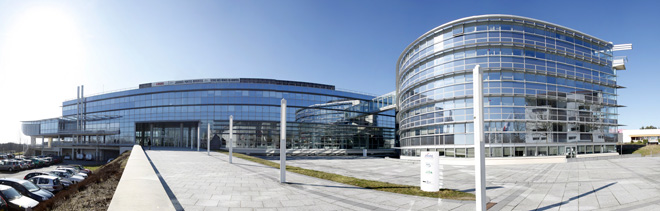
\includegraphics[scale=0.35]{ecole-mines-pano.jpg}}{}
\title[\bf Nantes, GDRE 2016]{\textbf{\large {Femtoscopy observables within NICA/MPD}}}

%\author[P.~Batyuk]{\textit{\textbf{{\footnotesize \underline{P.~Batyuk}, L.~Malinina (SINP MSU, JINR), \\ O.~Rogachevskiy (JINR)}}} \\
%  on behalf of the MPD collaboration}
\author[\bf P.~Batyuk]{\textit{\textbf{{\footnotesize \underline{P.~Batyuk}}}} \\
 on behalf of the MPD collaboration} 
\institute{\url{pavel.batyuk@jinr.ru}  \\ VBLHEP, JINR}

 \date{{\textbf{July 7, 2016}}}  
% \newpage \footnotesize April 14, 2016}}
  
\lstset{
%    frame=tb, % draw a frame at the top and bottom of the code block
    tabsize=4, % tab space width
    showstringspaces=false, % don't mark spaces in strings
 %   numbers=left, % display line numbers on the left
    commentstyle=\color{blue}, % comment color
    keywordstyle=\color{blue}, % keyword color
    stringstyle=\color{red} % string color
}

    
\begin{document}
\maketitle

\begin{frame}
  \bf
  \frametitle{Outline}
  \begin{itemize}
  \item The NICA complex
  %\item Heavy-ion scientific programme @ NICA 
  \item Feasibility of femtoscopy studies @ NICA
  \item MPDROOT::FEMTOMPD and its application to the TTE-estimation.
  \item Conclusions
  \end{itemize}
  \note{
  On behalf of the MPD collaboration of Joint Institute for Nuclear Research (JINR), located in town of Dubna, I would like to present you a report on "Femtoscopy observables within NICA/MPD". 
  \\
  A brief content of the report is presented in slide. I will tell briefly about the accelerator complex NICA. Then, in the first part of my talk I will discuss a possibility of femtoscopy studies at NICA. The second part is related to a software specially developed for femtoscopy analysis within MPD which is considered now as the main experiment to be performed at the NICA complex. And, finally, some conclusions and outlook are presented.
  }
\end{frame}

\begin{frame}[shrink=40]
  \bf
  \frametitle{NICA Complex}
  \begin{columns}[c]
    \column{.40\textwidth}
    \begin{block}{\centering \bf General characteristics:}
      \centering  Beams - {\color{red}$p$, $d$ ... $^{197}Au^{79+}$} \\
      \centering  Collision energy: 
      \begin{columns}[c]
        \column{.49\textwidth}
        $\sqrt{s_{NN}}$ = {\color{red} 4 - 11} GeV
        \column{.49\textwidth}
        $E_{lab}$ =  {\color{red}1 - 6} AGeV
      \end{columns}
      Luminosity: {\color{red}$10^{27}~cm^{-2}s^{-1}$} (Au), {\color{red}$10^{32}$} (p)

    \end{block}
    \column{.40\textwidth}
    \begin{block}{\centering \bf Experiments:}
      \begin{itemize}
      \item 2 interaction points - {\color{red}MPD} and  {\color{red}SPD}
      \item Fixed target experiment -  {\color{red}BM@N}
      \end{itemize}
    \end{block}
  \end{columns}
  \begin{columns}[c]
   % \column{.05\textwidth}
    \column{.75\textwidth}
    \begin{block}{}
      \begin{figure}[H]
        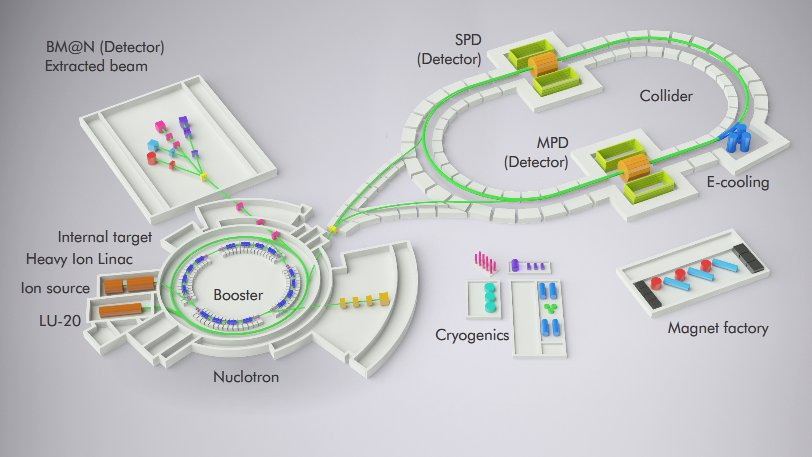
\includegraphics[width=1.\linewidth]{nica_complex1.png}
      \end{figure}
      \centering The general contractor is  {\color{red} STRABAG} (Bodostal-3 \& PCJ are the sub-contactors)
    \end{block}
    \column{.20\textwidth}
    \begin{block}{}
    \begin{itemize}
    \item {\color{red} 2017:} extracted beams of heavy ions are available within the BM@N experiment
    \item {\color{red} 2019}: a first configuration of the MPD setup available.
    \item {\color{red} 2023}: commissioning of the fully designed NICA-complex is foreseen.	
    \end{itemize}
 \end{block}

  \end{columns}
  \note{
    \footnotesize{
      NICA will be a new accelerator complex to be constructed at JINR and aimed to provide collider and fixed target  experiments with heavy ions up to gold at the maximum
      energy $\sqrt{s_{NN}}$ = 11 GeV. A schematic layout of the complex is shown in the slide. As I already mentioned, two types of experiments can be performed at the complex: collider and fixed target experiments.
      The last one called BM@N is functioning now in a test mode. 
      The NICA collider will have two points to be crossed by the beam at zero angle. There will be located two future collider experiments: SPD dedicated to some investigations in spin physics and the MPD. 
      According to the NICA project realization plan, in 2017 extracted beams of heavy ions will be available to start physics runs at the BM@N experiment. In 2019 the research program will be continued at higher energies with the MPD setup. In 2023 the commissioning of the fully design configuration of the NICA complex is considered to be done.
    }
  }
\end{frame}

%%%%%%%%%%%%%%%%%%%%%%%
\begin{comment}
\begin{frame}[shrink=40]
  \bf
  \frametitle{NICA heavy-ion programme}
  \begin{columns}[c]
    \column{.40\textwidth}
    \begin{block}{}
       \begin{figure}[H]
        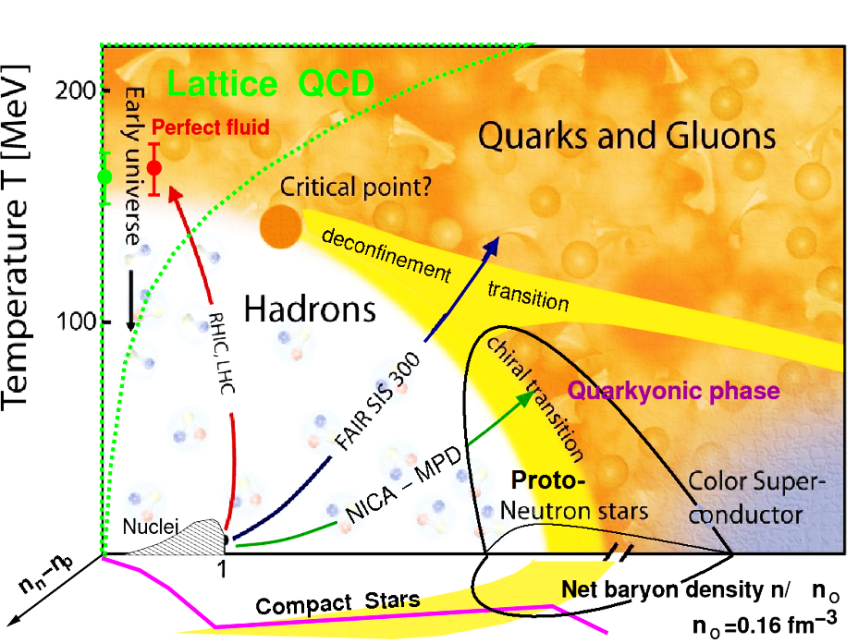
\includegraphics[width=1.0\textwidth]{qcd_diagram.png}
       \end{figure}
    \end{block}
    \column{.49\textwidth}
    \begin{block}{}
      \begin{itemize}
      \item Bulk properties, EoS
        \begin{itemize}
        \item {\color{red} particle yields \& spectra, ratios, femtoscopy, flow}
        \end{itemize}
      \item In-Medium modification of hadron properties
        \begin{itemize}
        \item {\color{red} onset of low-mass dilepton enhancement}
        \end{itemize}
      \item Deconfinement (chiral) phase transition at high $\rho_{b}$
        \begin{itemize}
        \item {\color{red} enhanced strangeness production  }
        \item {\color{red} Chiral Magnetic effect, $\Lambda$-polarization}
        \end{itemize}
      \item QCD Critical Point
        \begin{itemize}
        \item {\color{red} event-by-event fluctuations \& correlations}
        \end{itemize}
      \item Y-N interactions in dense nuclear matter
        \begin{itemize}
        \item {\color{red} hypernuclei}
        \end{itemize}
      \end{itemize}
    \end{block}
  \end{columns}

  \begin{columns}[c]
    \column{.49\textwidth}
    \begin{block}{\centering \bf QCD matter @ NICA:}
      \begin{itemize}
      \item  {\color{red} Highest (net-)baryon density ($\sqrt{s_{NN}} = 4 - 11$ GeV)}
      \item  {\color{red} The energy range brackets onset of deconfinement}
      \end{itemize}
    \end{block}

    \column{.49\textwidth}
     \begin{figure}[H]
       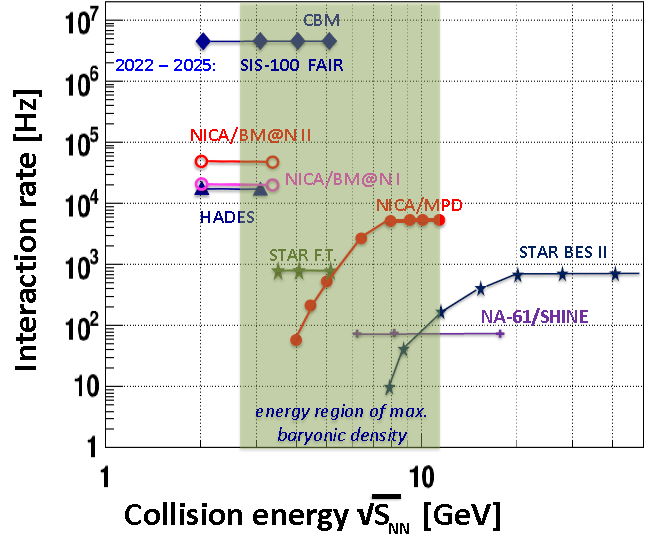
\includegraphics[width=0.75\textwidth]{interaction_rate.png}
       \end{figure}
  \end{columns}
  \note{ 
    \tiny{
      The main goal of physics program at the NICA complex is a search for the mixed phase of quark matter and baryon rich hadronic matter as a consequence
      of a 1PT. The current view of the QCD phase diagram is mostly an artistic view with only a few quantitative details from the available 
      experimental data or some QCD simulations on it. There are strong experimental evidences that the deconfined phase of nuclear matter QGP can be
      created in high energy nuclear collisions. As the collision energy is decreased down to several GeV per nucleon-nucleon pair, 
      there is a certain transition region of the collision energy below which it is no longer possible to access the plasma phase in the course of the collision. 
      Existing data on single particle spectra and mean multiplicities suggest that the transition occurs within the NICA energy
      range. Theoretical understanding of the transition between the hadronic phase and the plasma phase,
      and how it manifests itself in the nuclear collision observables, is still rather poor, and quantitative predictions cannot yet be made with a confidence. Furthermore, in addition to
      determining the existence and location of the transition region, where the new plasma phase is being created at the beginning, it is also interesting to
      establish a character of the associated phase transformation, whether it remains a smooth crossover, or
      becomes a first-order transition. In case of 1PT, the phase diagram must contain a critical point and its experimental identification forms a focal
      point for this research field. It has been suggested that the NICA experiments should concentrate on a variety of diagnostic
      observables to clarify the situation. Possible observables, presented in the slide, include particle yields and spectra,
      event-by-event fluctuations of multiplicity and transverse momentum of charged particles as well as the corresponding joint distributions.
    }
  }
\end{frame}
\end{comment}
%%%%%%%%%%%%%%%%%%%%%%%%%%%%%%%
\begin{frame}[shrink=25]
  \bf
  \frametitle{\centering \bf {\small MultiPurpose Detector (MPD) for $A + A$ collisions @ NICA}}
  \begin{columns}[c]
    \column{.4\textwidth}
    \begin{block}{\bf \centering Layout:}
      \begin{figure}[H]
        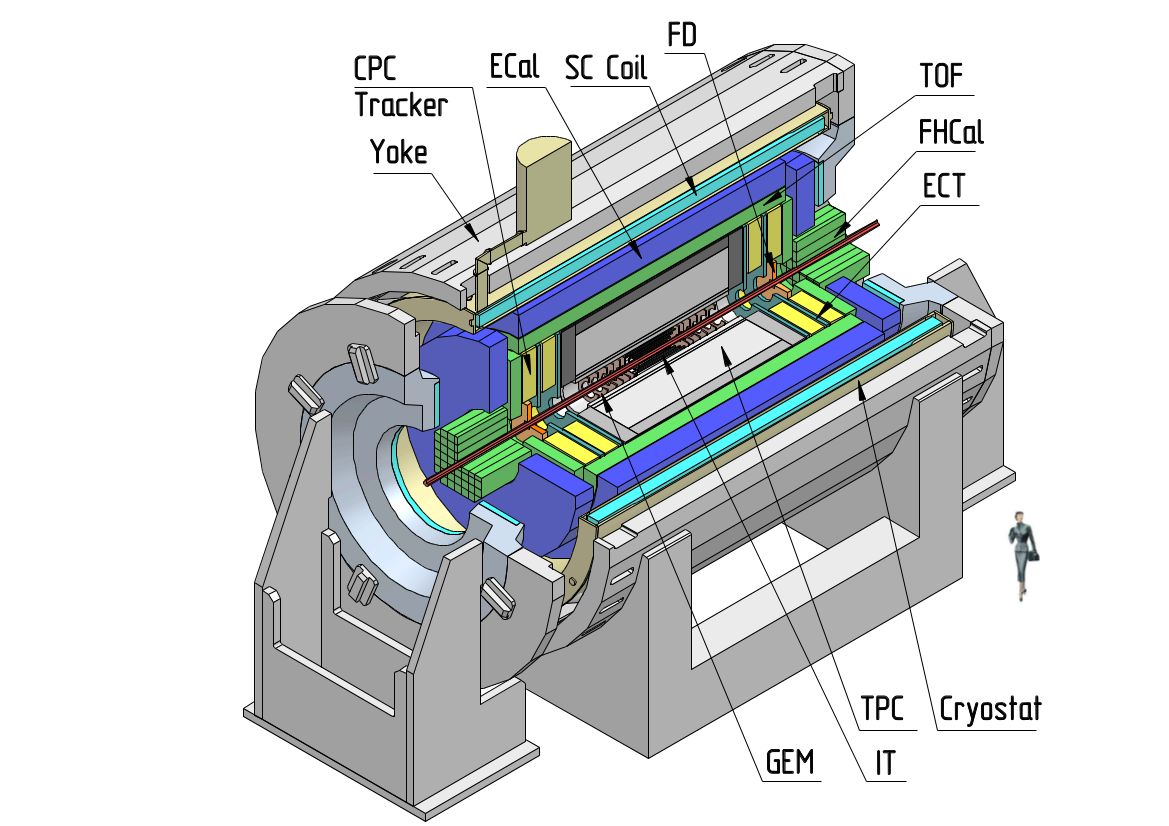
\includegraphics[width=.96\textwidth]{mpd.png}
      \end{figure}
    \end{block}
    \begin{block}{\bf \centering Momentum resolution:}
    \begin{figure}[H]
        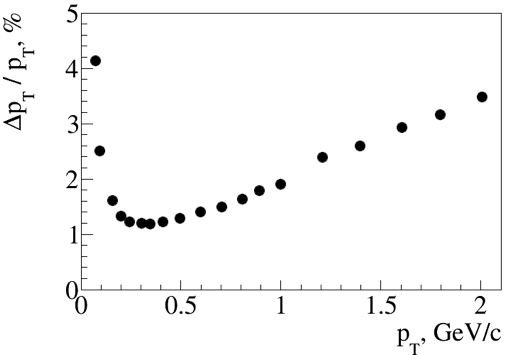
\includegraphics[width=.96\textwidth]{mom_res_mpd.png}
      \end{figure}    	
    \end{block}

    \column{.55\textwidth}
    \begin{block}{\bf \centering Benefits:}
      \begin{itemize}
      \item Hermeticity, $2\pi$-acceptance in azimuth
      \item 3D-tracking (TPC, ECT)
      \item Vertex high-resolution (IT)
      \item Powerful PID (TPC, TOF, ECAL)
        \begin{itemize}
        \item $\pi, K$ up to 1.5 GeV/c
        \item $K, p$ up to 3 GeV/c
        \item $\gamma, e$ from 0.1 GeV/c up to 3 GeV/c
        \end{itemize}
      \item Precise event characterization (FHCAL = ZDC) (centrality determination, reaction plane ...)
      \item Fast timing and triggering (FFD)
      \item Low material budget
      \item High event rate (up to 7 kHz) 
      \end{itemize}
    \end{block}
  \end{columns}
  \note{In slide a schematic layout of the MPD setup at the first stage of operation is shown. Some features of the setup are presented in the slide. The main ones are related to tracking procedure, PID and precise event characterization. Also, an example of the momentum resolution to be achieved is presented in the slide. 
}
\end{frame}

\begin{frame}[shrink=40]
  \bf
  \frametitle{\bf \centering Femtoscopy formalism}
  \begin{columns}[c]
    \column{.30\textwidth}
    \begin{block}{}
      \begin{figure}[H]
        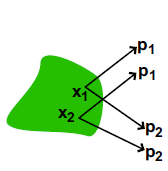
\includegraphics[width=1.\linewidth]{corr_femto1.png}
      \end{figure}
    \end{block}
    \column{.65\textwidth}
    \begin{block}{{\bf \centering Correlation femtoscopy:}}
 %     {\tiny
        Measurement of space-time characteristics $R$, $c_{\tau}$ (fm) of particle production
        using particle correlations due to the effects of quantum statistics (QS) and final state interactions (FSI)
%      }
    \end{block}
      \begin{block}{{\bf \centering Two-particle correlation function:}}
%      \tiny{
        \begin{center}
          {\bf theory:     $C(q) = \dfrac{N_{2}(p_{1}, p_{2})}{N_{1}(p_{1}) N_{2}(p_{2})}, C(\infty) = 1$
        
            experiment: $C(q) = \dfrac{S(q)}{B(q)}, q = p_{1} - p_{2}$
            
            \alert {S(q)} is a distribution of pair momentum difference of particles from the same event
            
            \alert {B(q)} is a reference distribution built by mixing of particles from different events}
        \end{center}
 %     }
    \end{block}
  \end{columns}

  \begin{columns}[c]
    \column{.45\textwidth}
    \begin{block}{\bf \centering Parametrizations used:}     
     \begin{block}{\bf \centering 1D CF:}
      \centering {
        $C(q) = 1 + \lambda e^{-R_{inv}^{2} q_{inv}^{2}}$
      }

      \small {\alert{1d-analysis}} is sensitive only to the system size averaged over all directions.
    \end{block}
    \begin{block}{\bf \centering 3D CF:}
    \centering {
      $C(q) = 1 + \lambda e^{-R_{out}^{2}q_{out}^{2} - R_{side}^{2}q_{side}^{2} - R_{long}^{2}q_{long}^{2}}$
    }
    
    \small {\alert{3d-analysis}} gives an access to the three system sizes in three directions separately.
    \end{block}
    \end{block}
    \column{.49\textwidth}
    \begin{block}{\center \bf Definition of femtoscopy radii:}
    \begin{figure}[H]
      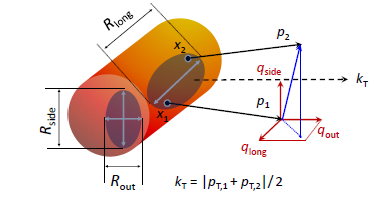
\includegraphics[width=.9\linewidth]{corr_femto4.png}
    \end{figure}
  \end{block}
  \end{columns}
  \note{
    {Well, in this slide the femtoscopy formalism is presented in a brief manner. Since it is well known for everyone in the auditory, I will not stop here and go further.}
  }
\end{frame}

\begin{frame}
  \frametitle{\bf \centering Motivation}
  \begin{columns}[c]
    \column{.48\textwidth}
    \begin{block}{}
      \bf Crossover transition to QGP occurs at RHIC \& LHC
    \end{block}
    \begin{block}{}
      \begin{figure}[H]
        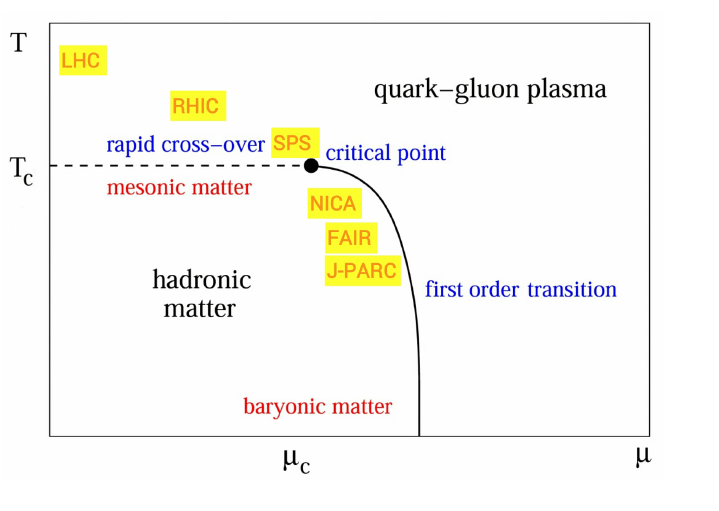
\includegraphics[width=1.\linewidth]{corr_femto5.png}
      \end{figure}
    \end{block}
    \column{.48\textwidth}
    \begin{block}{\centering \bf Questions to be answered:}
      {\bf 
       \begin{itemize}
   %    \item 1st order phase transition (PT) to the QGP occurs at lower energies(?)     
       \item What femtoscopy observables are the most sensitive to this difference?
       \item At what energies do the hydro models with a first order phase transition (1PT) describe femtoscopy observables better than those with crossover?
       \end{itemize}
       }
     \end{block}
  \end{columns}
  \note{
      The regime obtained at the performed experiments at the highest RHIC and LHC energies, according to the lattice QCD calculations, corresponds to a rapid, smooth crossover at large temperature T and vanishing values of baryonic chemical potential $\mu_{B}$. At the same time, various models predict a strong first order phase transition at low and moderate temperatures and large values of $\mu_{B}$. Since we try to locate a certain region, where type of the phase transition is changed, by femtoscopy tools, the following questions concretize a problem to be solved:
      \begin{enumerate}
      	\item What femtoscopy observables are the most sensitive to this difference?
        \item At what energies do the hydro models with a first order phase transition (1PT) describe femtoscopy observables better than those with crossover?
      \end{enumerate}
  }
\end{frame}

\begin{frame}
  \bf
  \frametitle{Femtoscopy: from high to low energies...}
  \begin{columns}
    \column{.48\textwidth}
    \begin{block}{}
      \footnotesize{
        \begin{center}
          \bf
          RHIC: $\sqrt{s_{NN}}$ = 62 to 200 GeV
          
          \vspace{0.15cm}
          
          \alert {large T \& small $\mu_{B}$}

          \vspace{0.15cm}
          
          % {\tiny New state of matter, the strongly coupled Quark Gluon Plasma (sQGP)}

          \vspace{0.15cm}
          
          \alert {Smooth, rapid crossover}

        \end{center}
      }
    \end{block}
    
    \begin{block}{}
      \footnotesize{
        \begin{center}
          \bf
         BES @ RHIC: $\sqrt{s_{NN}}$ = 7.7, 11.5, 19.6, 27, 39 GeV

        \vspace{0.2cm}
        
        \alert {small T \& large $\mu_{B}$}

        \vspace{0.15cm}
        
       % {\tiny search for ``critical point''}

        \vspace{0.15cm}
      
        %\alert {1st order phase transition}
        \alert{search for ``critical point''}
         \end{center}
      }
    \end{block}
    \begin{block}{}
      \footnotesize{
        \begin{center}
          \bf
          NICA: $\sqrt{s_{NN}}$ = 4 to 11 GeV

           \vspace{0.15cm}
        
           \alert {small T \& large $\mu_{B}$}

        \end{center} 
      }
    \end{block}
    \begin{block}{}
      {\centering \footnotesize \bf \alert {What do the modern  hydrodynamic (hybrid) models expect?}}
    \end{block}   
    \column{.4\textwidth}
    \begin{block}{\center \tiny \bf STAR, Phys.Rev. C92 (2015) 1, 014904}
      \begin{figure}[H]
        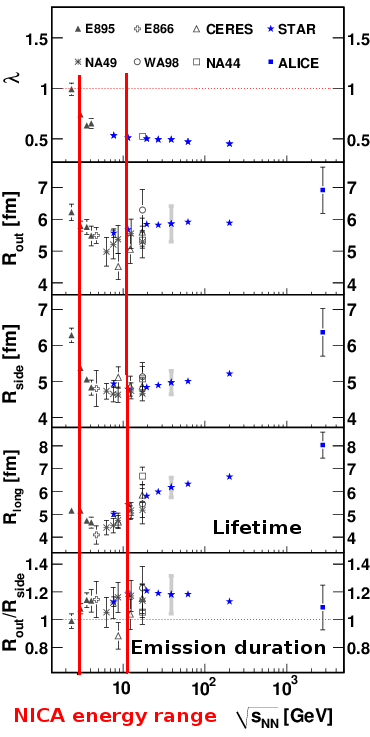
\includegraphics[width=.65\linewidth]{RiRootS.png}
      \end{figure}
    \end{block}
  \end{columns}
  \note{
In slide the regimes obtained at the highest RHIC energies and BES are presented. In Fig., representing a dependence of the femtoscopy radii on energy from different experiments, an energy scale, corresponded to the NICA energies, is presented by two red lines. In this energy range $R_{long}$ and ratio of $R_{out}$ to $R_{side}$ reveal a non-monotonous behavior that could be interesting for a detailed study.
  }
\end{frame}

\begin{frame}[shrink=50]
  \frametitle{vHLLE + UrQMD model}
   \begin{block}{{ \bf Iu. Karpenko, P. Huovinen, H.Petersen, M. Bleicher, Phys.Rev. C 91, 064901 (2015) \\
    vHLLE code: free and open source, https://github.com/yukarpenko/vhlle}}
    \begin{figure}[H]
      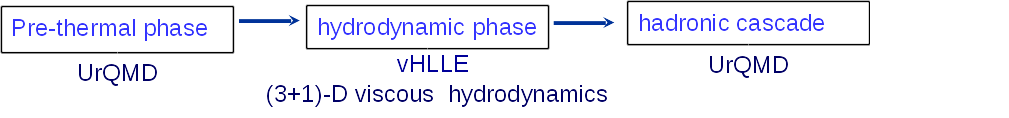
\includegraphics[width=1.\linewidth]{vHLLE.png}
    \end{figure}
  \end{block}

    
 \begin{columns}[c]
 \column{.60\textwidth}
  \begin{block}{}
    \begin{figure}[H]
      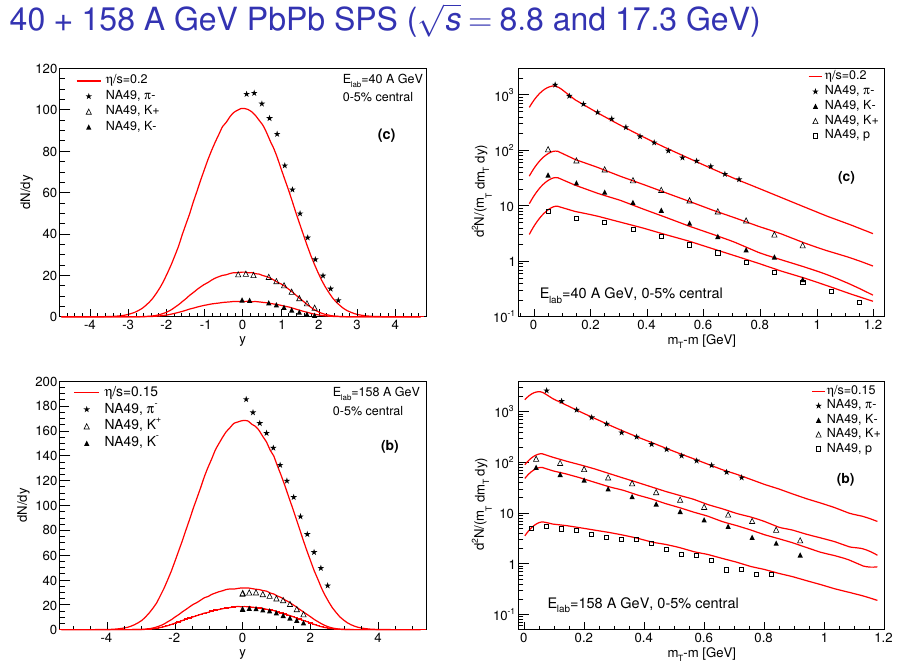
\includegraphics[width=1.\linewidth]{vhlle_calibr.png}
    \end{figure}
  \end{block}
  \column{.35\textwidth}
   \begin{block}{}
       { \bf \center Chiral EoS - \alert{crossover} \\}
       { \bf J. Steinheimer et al, J. Phys. G 38, 035001 (2011)}
     \end{block}
      \begin{block}{}
        {\bf \center HadronGas + Bag Model - \alert{1PT} \\}
        { \bf P. F. Kolb et al, Phys.Rev. C 62, 054909 (2000)}
     \end{block}

  \begin{block}{}
  \bf {\color{blue} More details in the report of D.~Wielanek (GDRE 2016)}	
  \end{block}
  \end{columns}
  \note{
     In order to answer the formulated questions the hybrid vHLLE + UrQMD model was chosen as a candidate. It includes three phases: pre-thermal phase, realized via UrQMD, hydrodynamics phase and hadronic cascade, realized via UrQMD also. We tried to use pure UrQMD3.4 with hydro and without, PHSD and other models, but they do not describe on a reasonable level existing femtoscopy data. More details about the model you can find in the report of D.~Wielanek to be presented after me.
       }
\end{frame}

\begin{frame}[shrink=20]
  \frametitle{vHLLE + UrQMD model}
  \begin{block}{{ \bf {\footnotesize Iu. Karpenko, P. Huovinen, H.Petersen, M. Bleicher, Phys.Rev. C 91, 064901 (2015)} \\
    vHLLE code: free and open source, https://github.com/yukarpenko/vhlle}}
    \begin{figure}[H]
      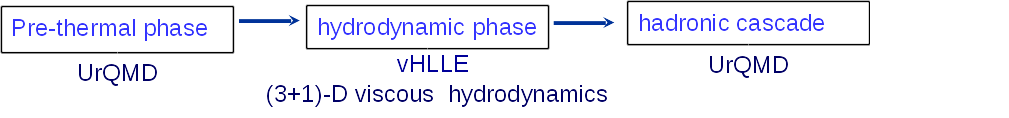
\includegraphics[width=1.\linewidth]{vHLLE.png}
    \end{figure}
  \end{block}
  \begin{columns}[c]
    \column{.30\textwidth}
        \begin{block}{\bf \centering AuAu @ $\sqrt{s_{NN}} = 11.5$ GeV, pions:}
        \begin{figure}[H]
          %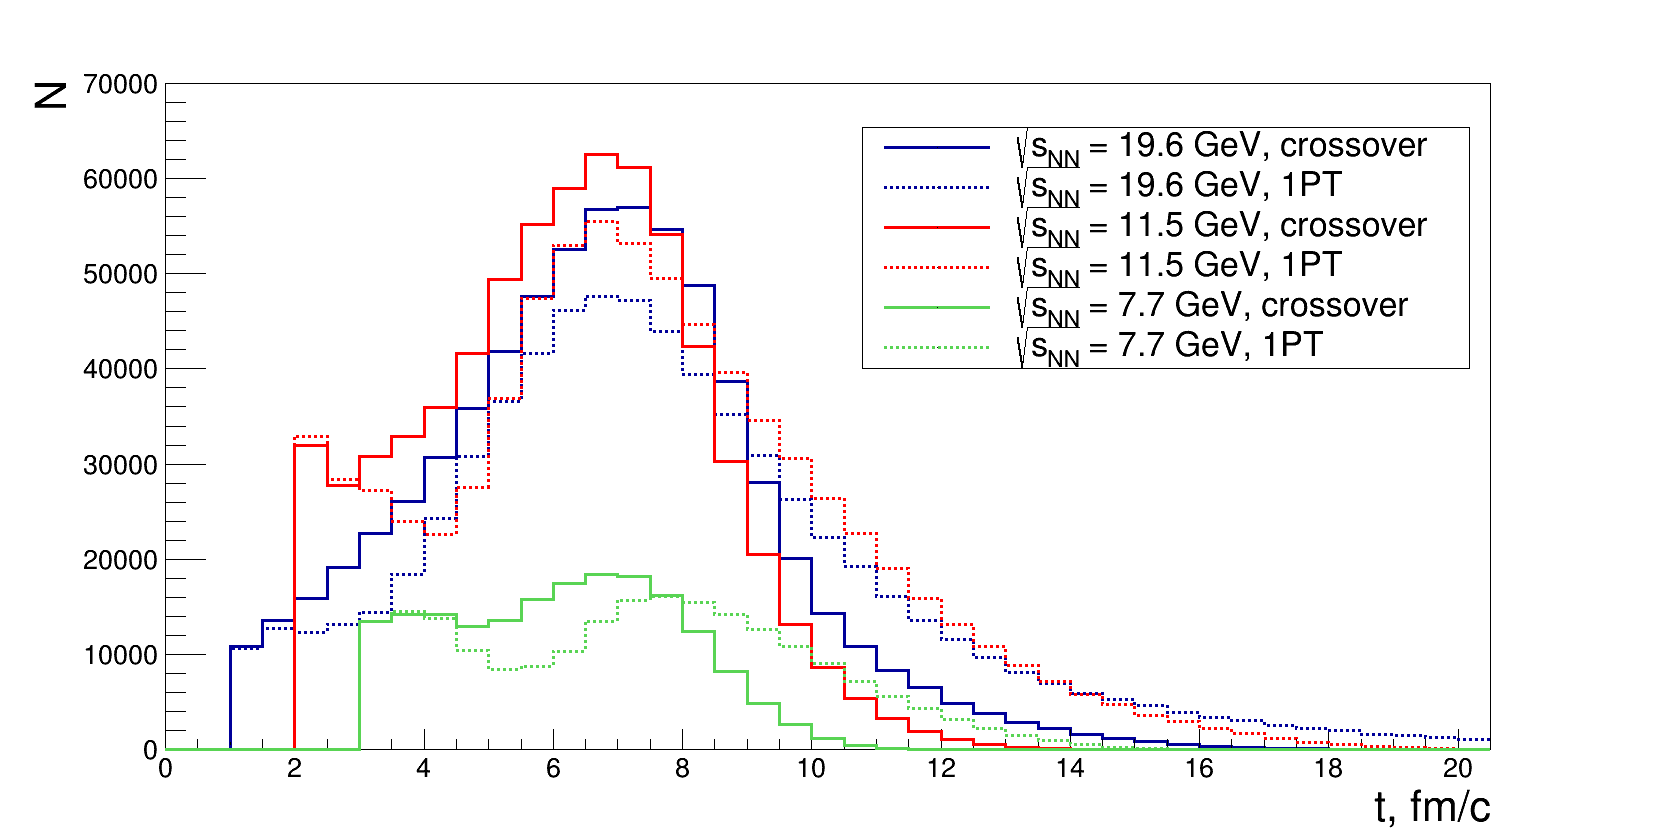
\includegraphics[width=.95\linewidth]{vHLLE_tfr.png}
          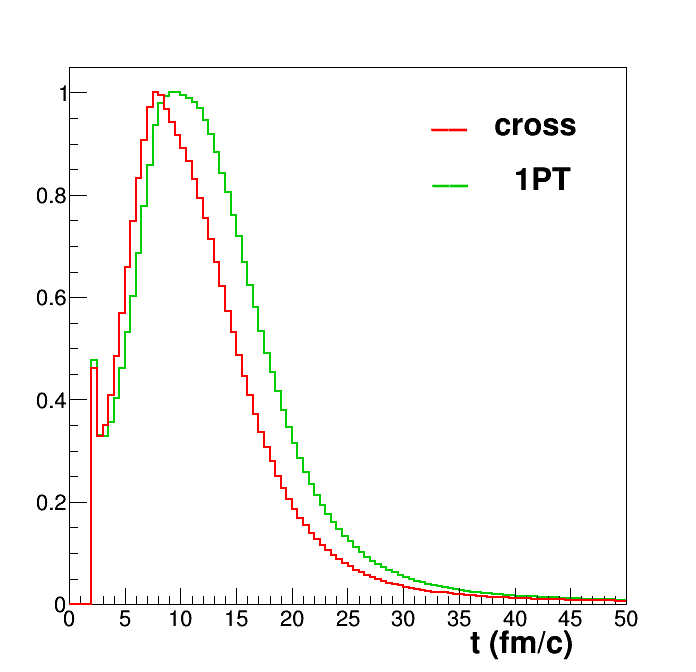
\includegraphics[width=.95\linewidth]{time_11GeV_pions.png}
        \end{figure}
     \end{block}
     \column{.30\textwidth}
         \begin{block}{\bf \centering AuAu @ $\sqrt{s_{NN}} = 11.5$ GeV, kaons:}
        \begin{figure}[H]
          %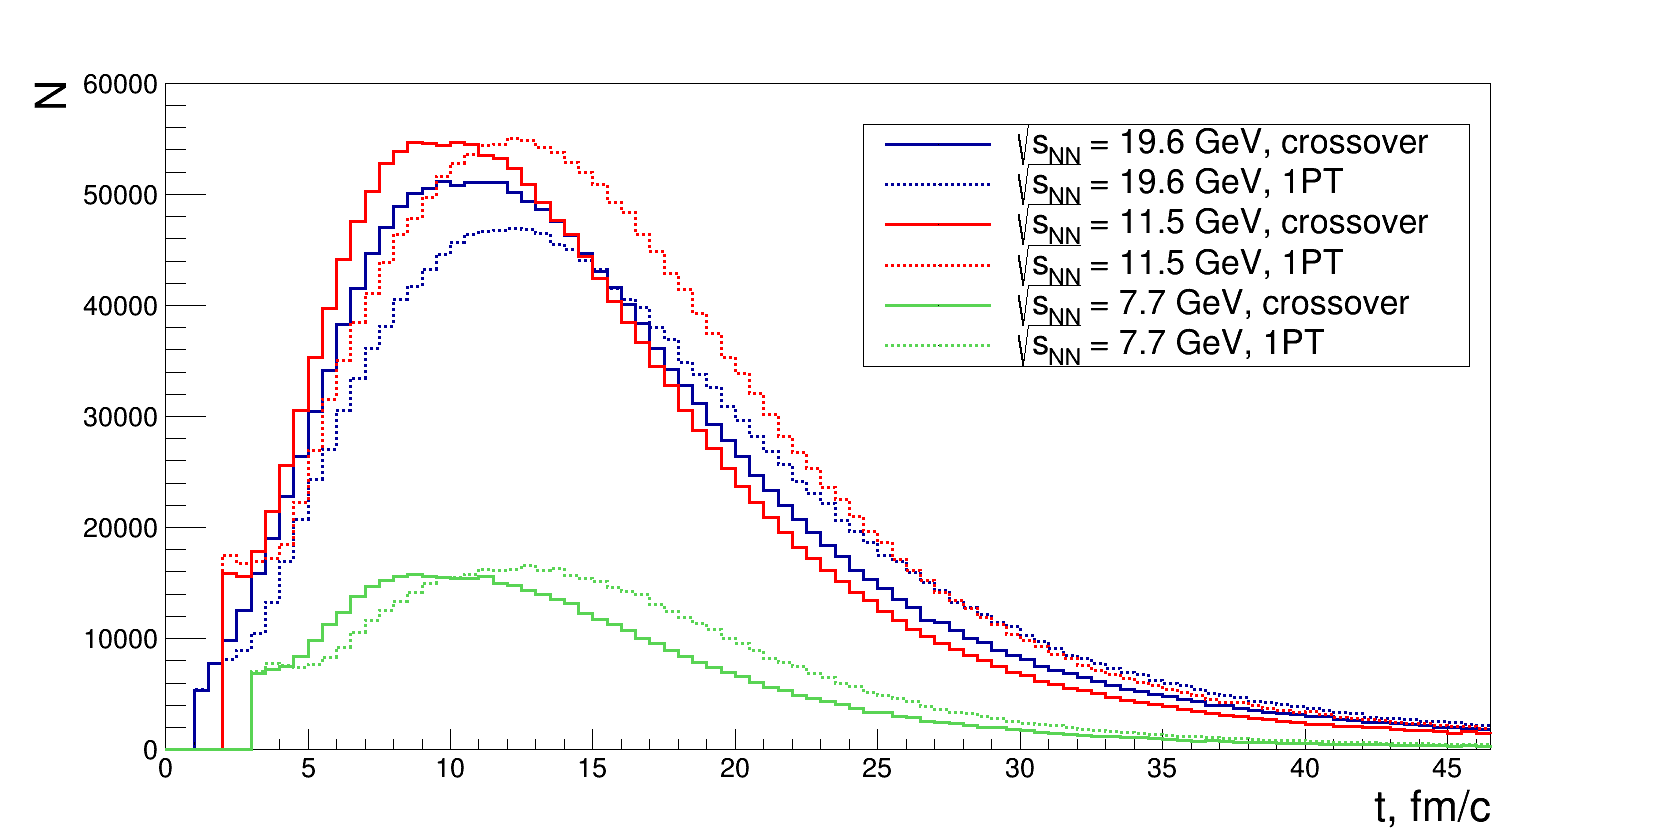
\includegraphics[width=.95\linewidth]{vHLLE_UrQMD_tfr.png}
        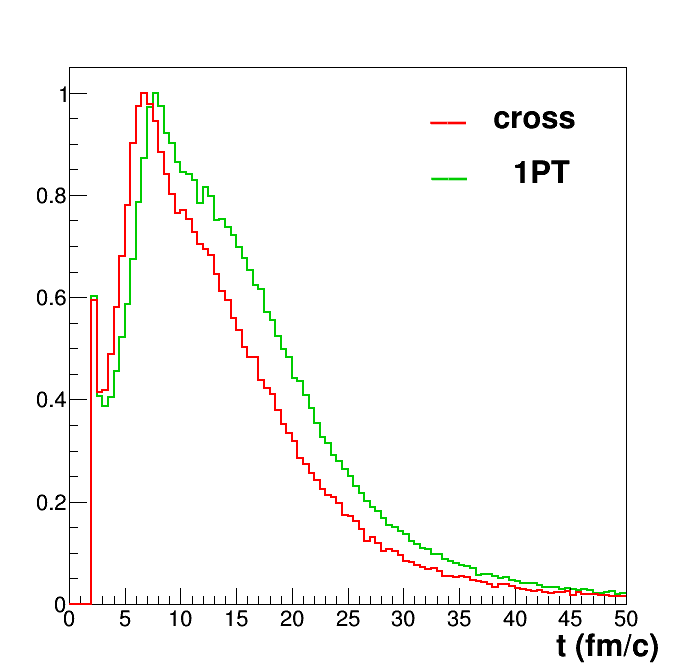
\includegraphics[width=.95\linewidth]{time_11GeV_kaons.png}  
        \end{figure}
     \end{block}
     \column{.30\textwidth}
     \begin{block}{}
      \bf \centering 
        %{\color{red} Hydro phase lasts longer with 1PT}.
        1PT delays emission of particles.
        Is it possible to see this time difference using the femtoscopy techniques?
    \end{block} 
  \end{columns}
  \note{
  In Fig. time emission of pions and kaons, derived from the model, is presented. One can see a time difference in emission depending on the EoS used: the 1PT delays emission of particles with respect to the crossover. So, is it possible to see the time difference using the femtoscopy techniques?
  }
\end{frame}

%
\begin{frame}[shrink=50]
\frametitle{{\small \bf \centering Projections of 3D CF in comparison of the two EoS's used}}
  \bf 
  \begin{columns}
  \column{.48\textwidth} 
  \begin{block}{\bf \centering Pions:}
  	\begin{figure}[H]
  	 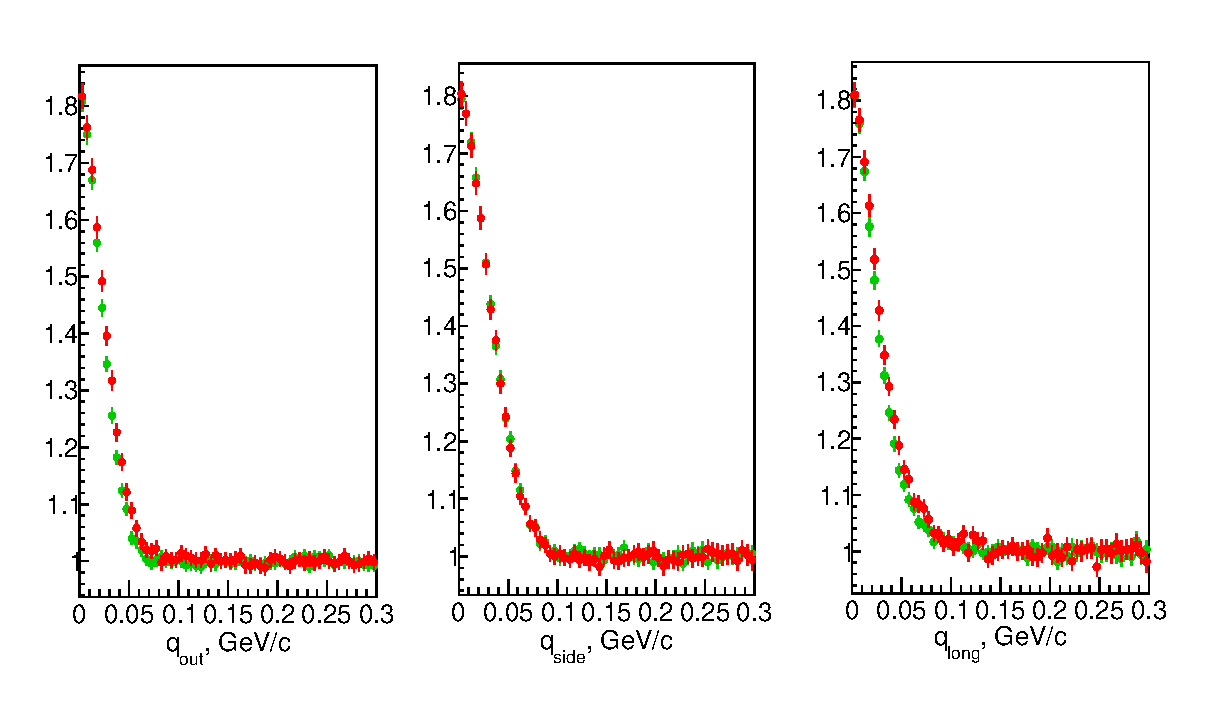
\includegraphics[width=.95\textwidth]{pions_1PT_crossover_comparison.eps}
    \end{figure}	
  \end{block}
  \begin{block}{\bf \centering Kaons:}
  	\begin{figure}[H]
      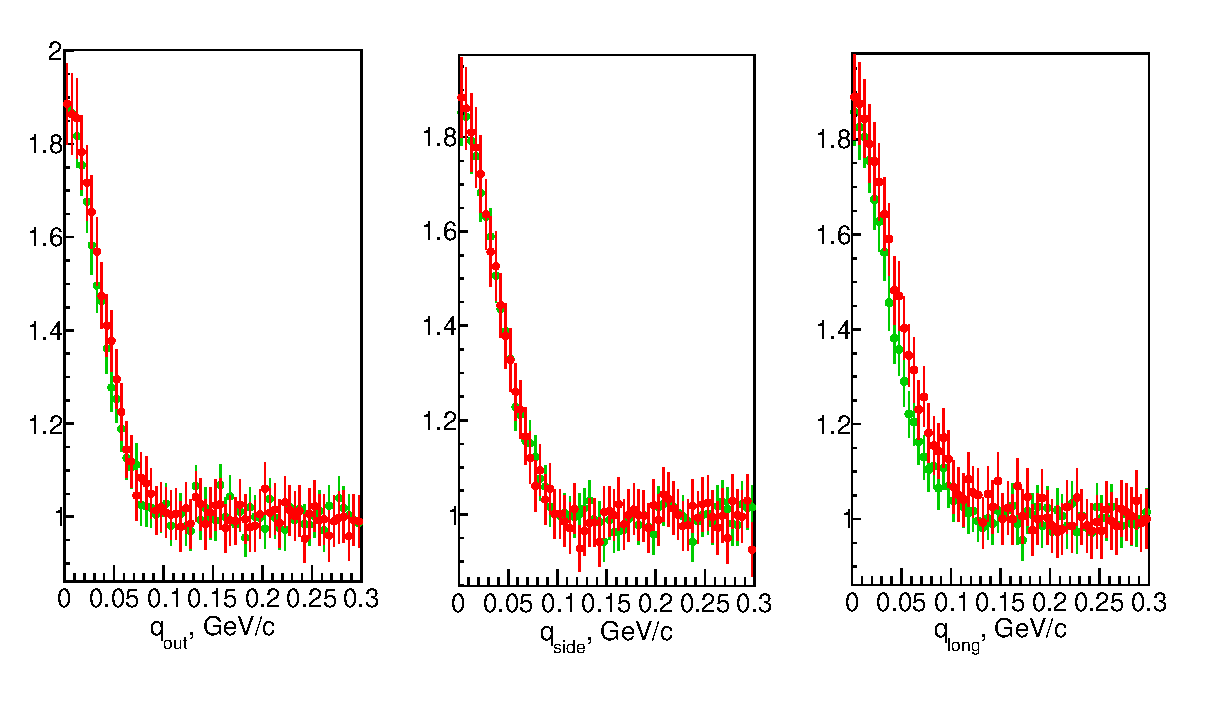
\includegraphics[width=.95\textwidth]{kaons_1PT_crossover_comparison.eps}
    \end{figure}
  \end{block}
 \column{.48\textwidth}
\begin{block}{}
\begin{itemize}
\item {\color{LimeGreen} Green line} --> EoS: 1PT \\
{\color{red} Red line} --> EoS: crossover
\item Each projection is extracted while other directions are fixed in the corridor \underline {5 MeV/c for pions} and \underline {15 MeV/c for kaons}.	
\end{itemize}
\end{block}

\begin{block}{}
    Pions:
    \begin{figure}[H]
         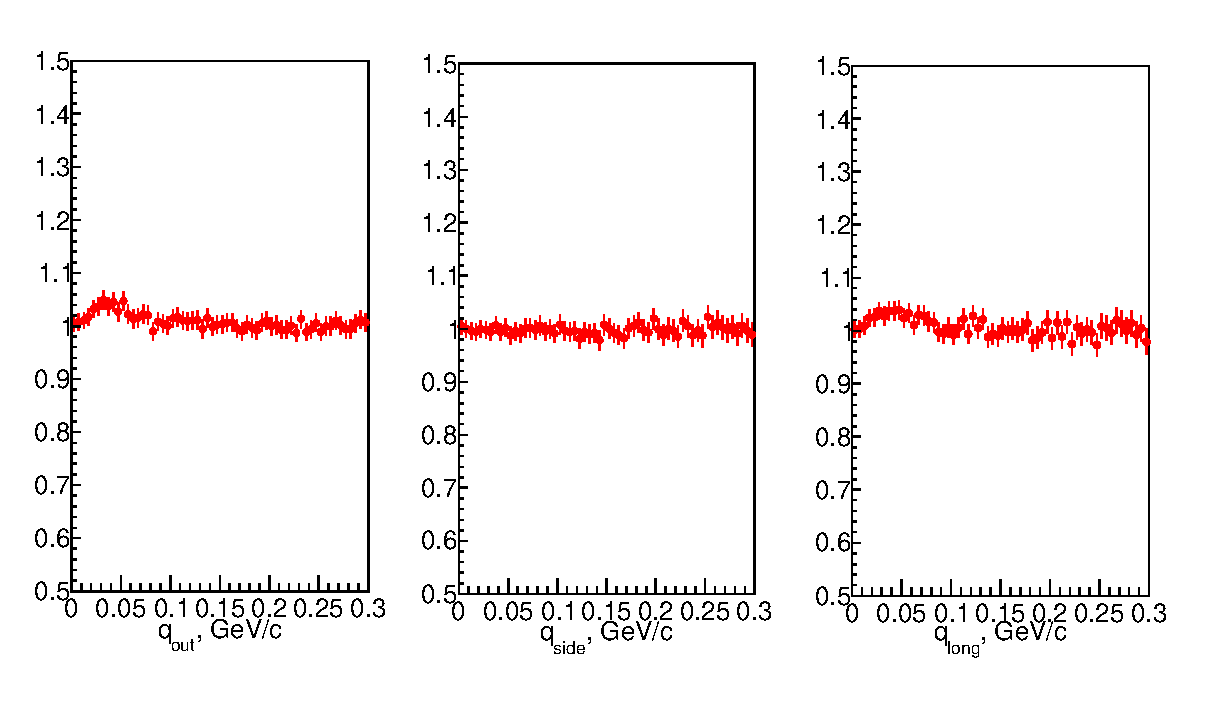
\includegraphics[width=.7\linewidth]{ratios_pions.eps}
    \end{figure}
    Kaons:
	\begin{figure}[H]
         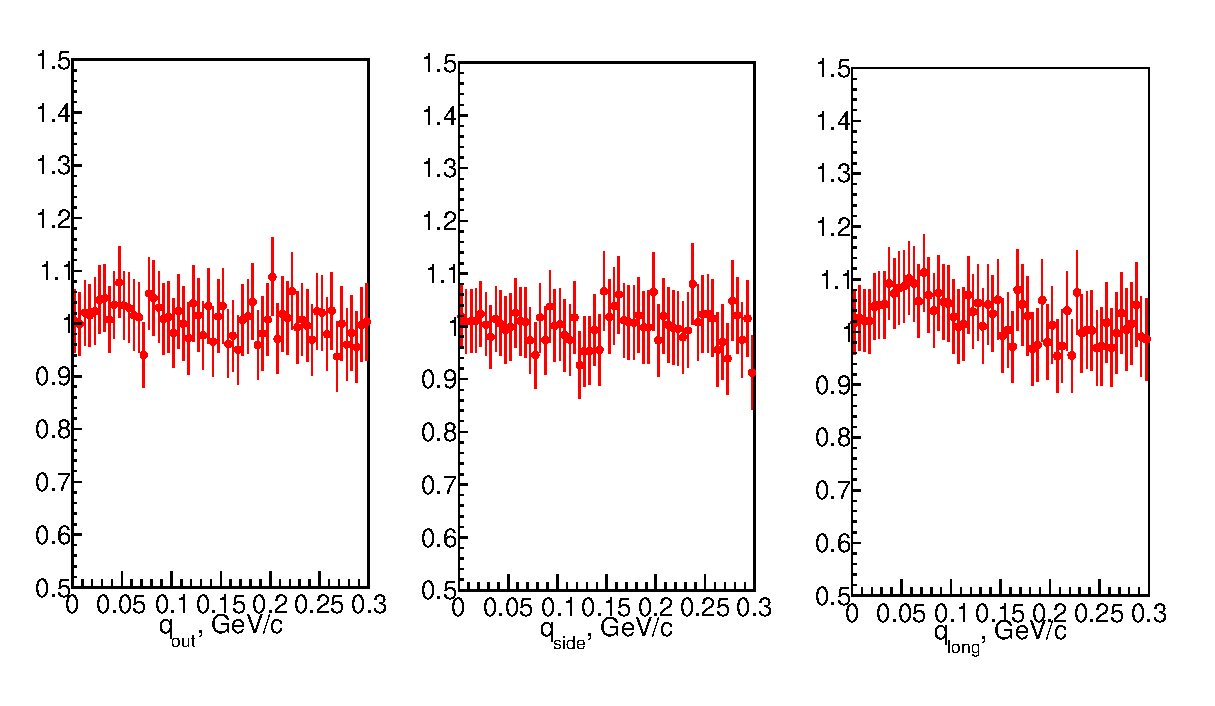
\includegraphics[width=.7\linewidth]{ratios_kaons.eps}
    \end{figure}
\end{block}
\begin{block}{}
Visible difference in out- and long-directions is clearer for kaons.
\end{block}
\end{columns}
\note{
In Fig. projections of 3D CFs on out-, side- and long-directions are presented for pions and kaons. Each projection is extracted while other directions are fixed in the corridor of 5 MeV/c for pions and 15 MeV/c for kaons. A certain difference between the two EoS used is observed in the projections, especially, in side- and long-directions. In order to see an approximate magnitude of the difference, the corresponding ratios are plotted. One can see that maximal magnitude is close to 3-5\% for pions and about 10\% for kaons and observed at small values of q. Probably, 3D CFs look sensitive to type of the EoS used and the fact is considered as an observable we are looking for. 
}
\end{frame}

\begin{frame}[shrink=10]
  \frametitle{Source Function Technique}
  \begin{columns}
    \column{.48\textwidth}
    \begin{block}{}
      $S(r^{*})$ is a {\bf source function}, which represents time-integrated distribution of particle emission points separation
      $r^{*}$ in the PRF.
    \end{block}
     \begin{block}{}
       $C({\bf q}) - 1 \equiv R({\bf q}) = \int (|\phi({\bf q, r})|^{2} - 1) S({\bf r}) d{\bf r}$
     \end{block}
      \begin{block}{}
        The method is suitable for extracting the $S(r^{*})$ directly from the data {\bf {\color{red}without any hypothesis about source shape}}.
       
    \end{block}
    \column{.48\textwidth}
     \begin{block}{\centering {\tiny \bf STAR, Phys.Rev. C88 (2013) 3, 034906}}
       \begin{figure}[H]
         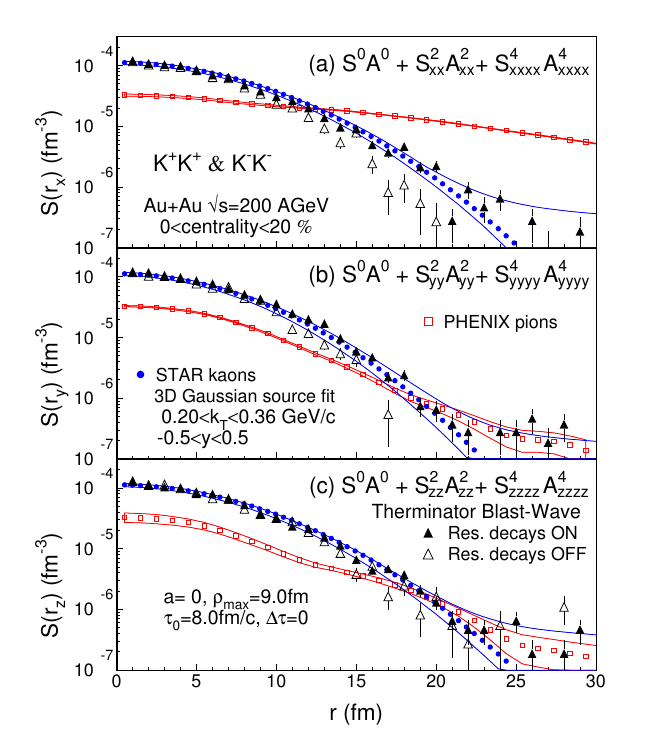
\includegraphics[width=.95\linewidth]{source_func.png}
       \end{figure}
     \end{block}
  \end{columns}
  \note{
    To obtain a more detailed information on the space-time structure of the system, one can use more complicated parameterizations accounting for non-Gaussian tails, or exploit the source imaging technique. The technique is based on Fourier-like extraction of the emission function from the measured correlation function in the PRF. In case of an arbitrary (non-Gaussian) source function, using this technique, it is possible to see the detailed source structure, which can likely deviate from the Gaussian distribution, having a more complicated shape without any hypothesis about source shape.   
}
\end{frame}

\begin{frame}[shrink=40]
  \frametitle{{\small \bf \centering Projections of Source Function, pions (calculated in the PRF)}}
  \begin{columns}
    \column{.48\textwidth}
    \begin{block}{\bf  \centering AuAu @ $\sqrt{s_{NN}} = 7.7$ GeV, vHLLE}
      \begin{figure}[H]
         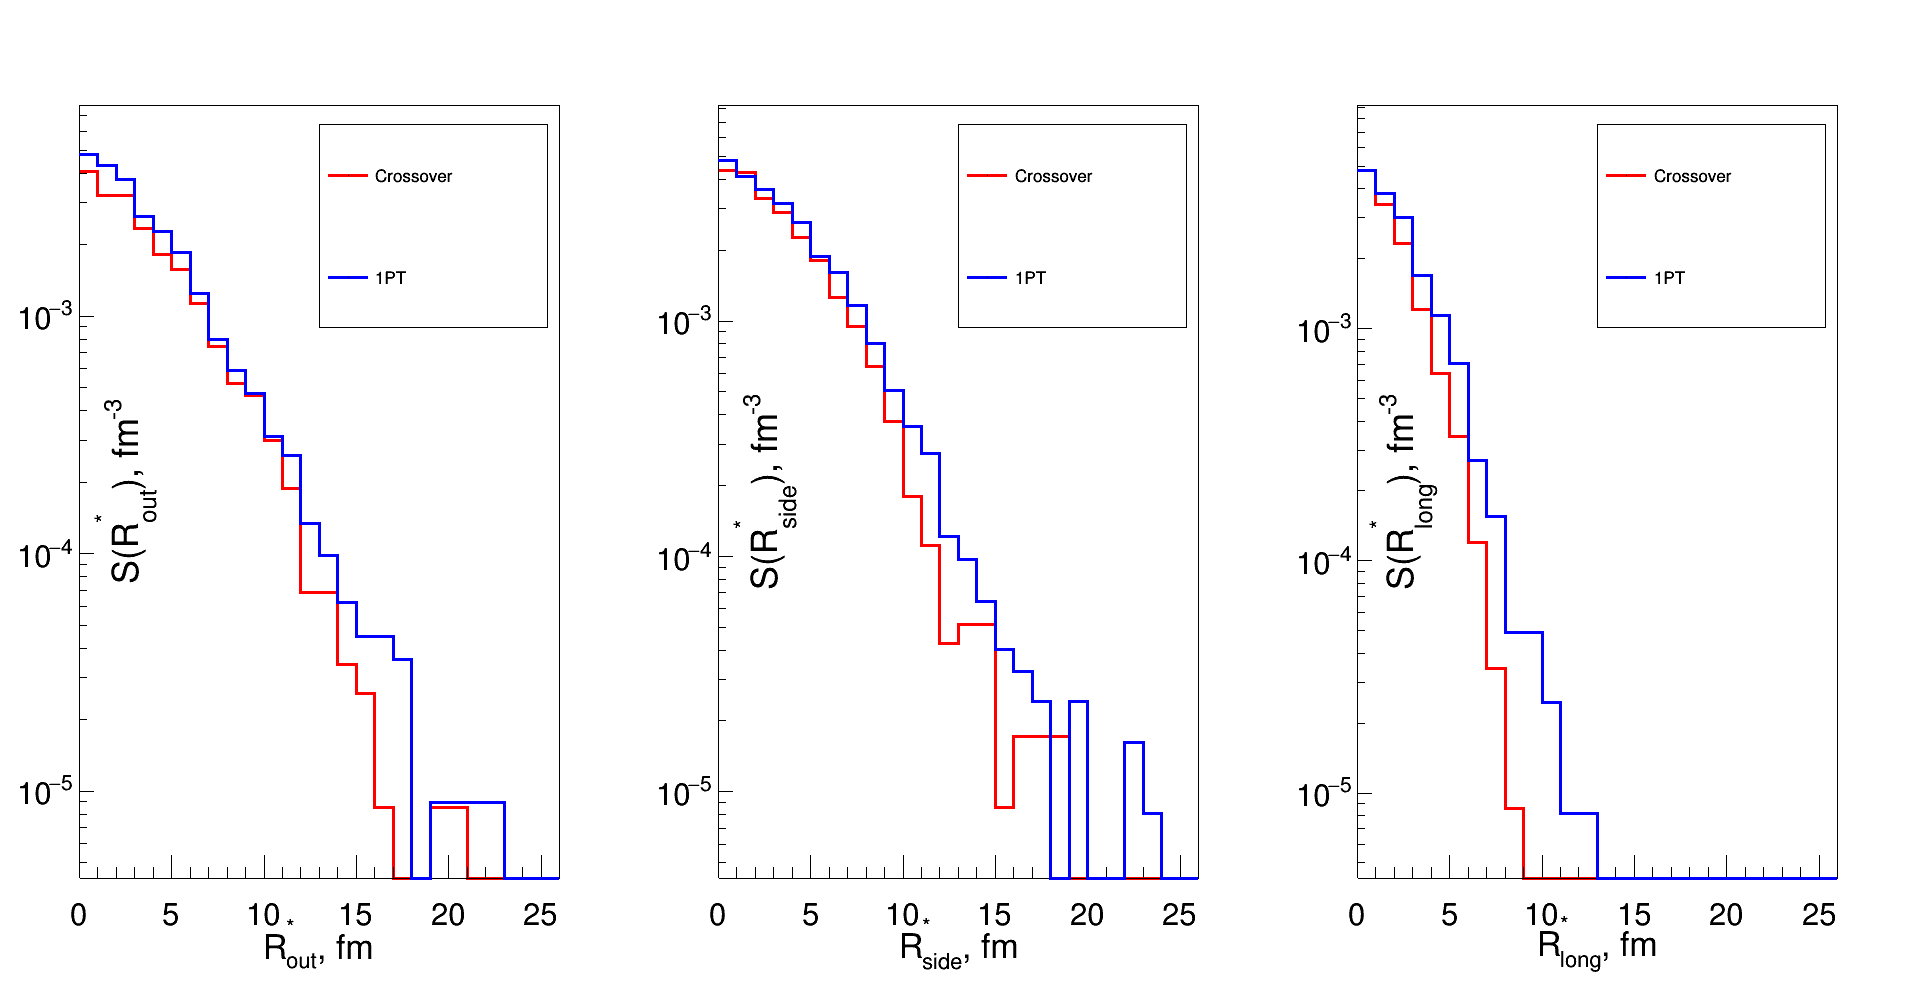
\includegraphics[width=1.\linewidth]{SF_vHLLE_77gev.png}
      \end{figure}
    \end{block}
    \begin{block}{\bf  \centering AuAu @ $\sqrt{s_{NN}} = 7.7$ GeV, vHLLE + UrQMD}
      \begin{figure}[H]
        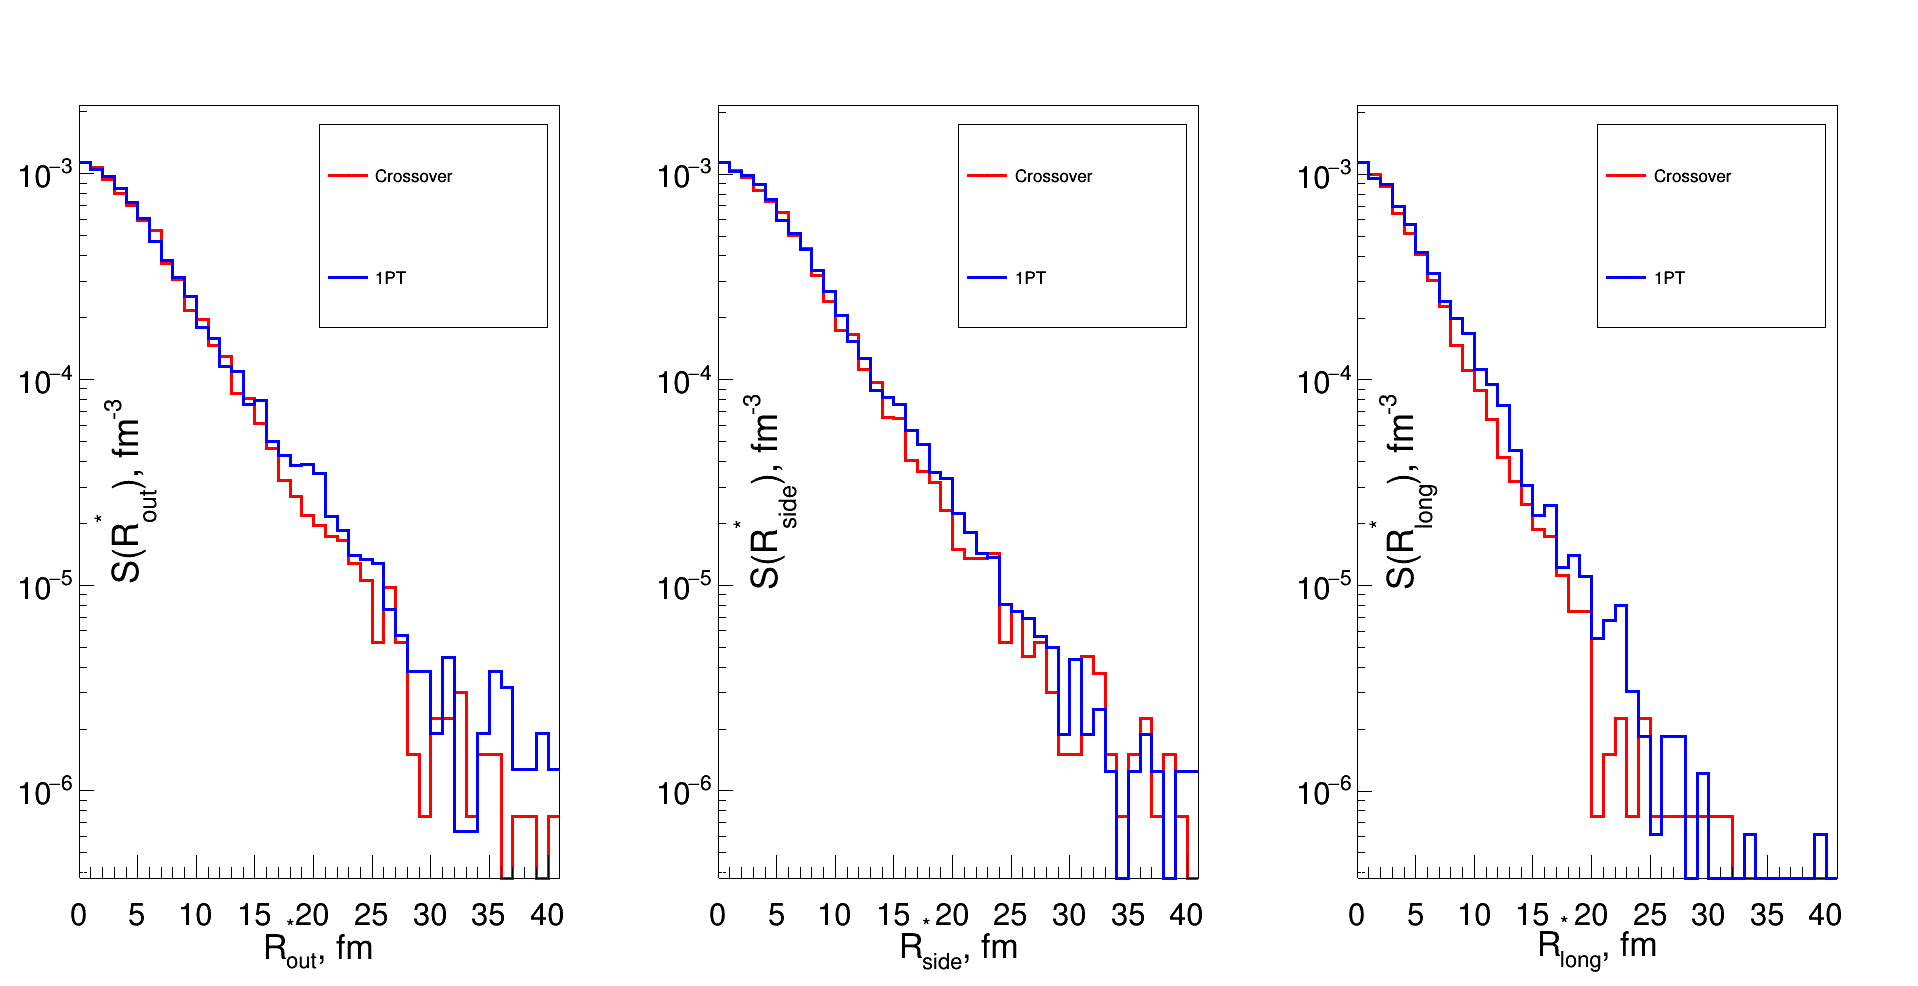
\includegraphics[width=1.\linewidth]{SF_vHLLE_UrQMD_77gev.png} \\
      \end{figure}
    \end{block}
    \column{.48\textwidth}
     \begin{block}{\bf \centering AuAu @ $\sqrt{s_{NN}} = 11.5$ GeV, vHLLE}
       \begin{figure}[H]
         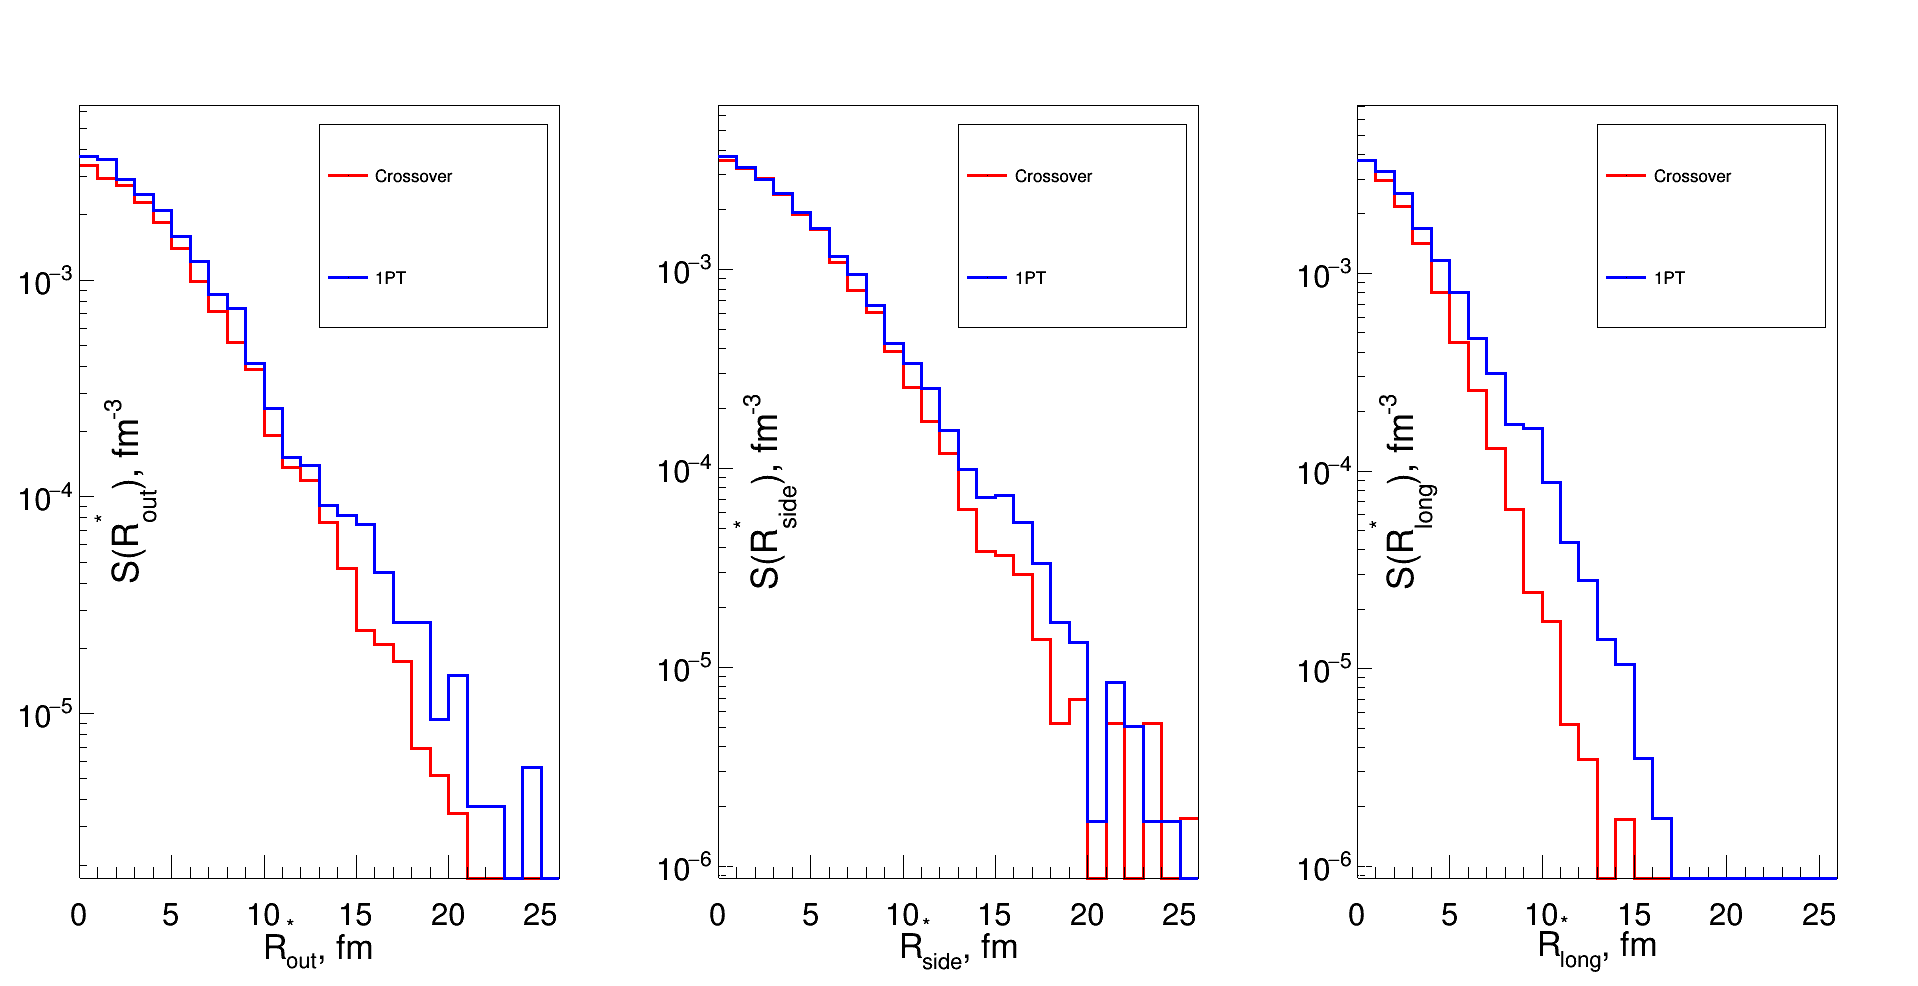
\includegraphics[width=1.\linewidth]{SF_vHLLE_115gev.png}
       \end{figure}
    \end{block}
    \begin{block}{\bf \centering AuAu @ $\sqrt{s_{NN}} = 11.5$ GeV, vHLLE + UrQMD}
      \begin{figure}[H]
         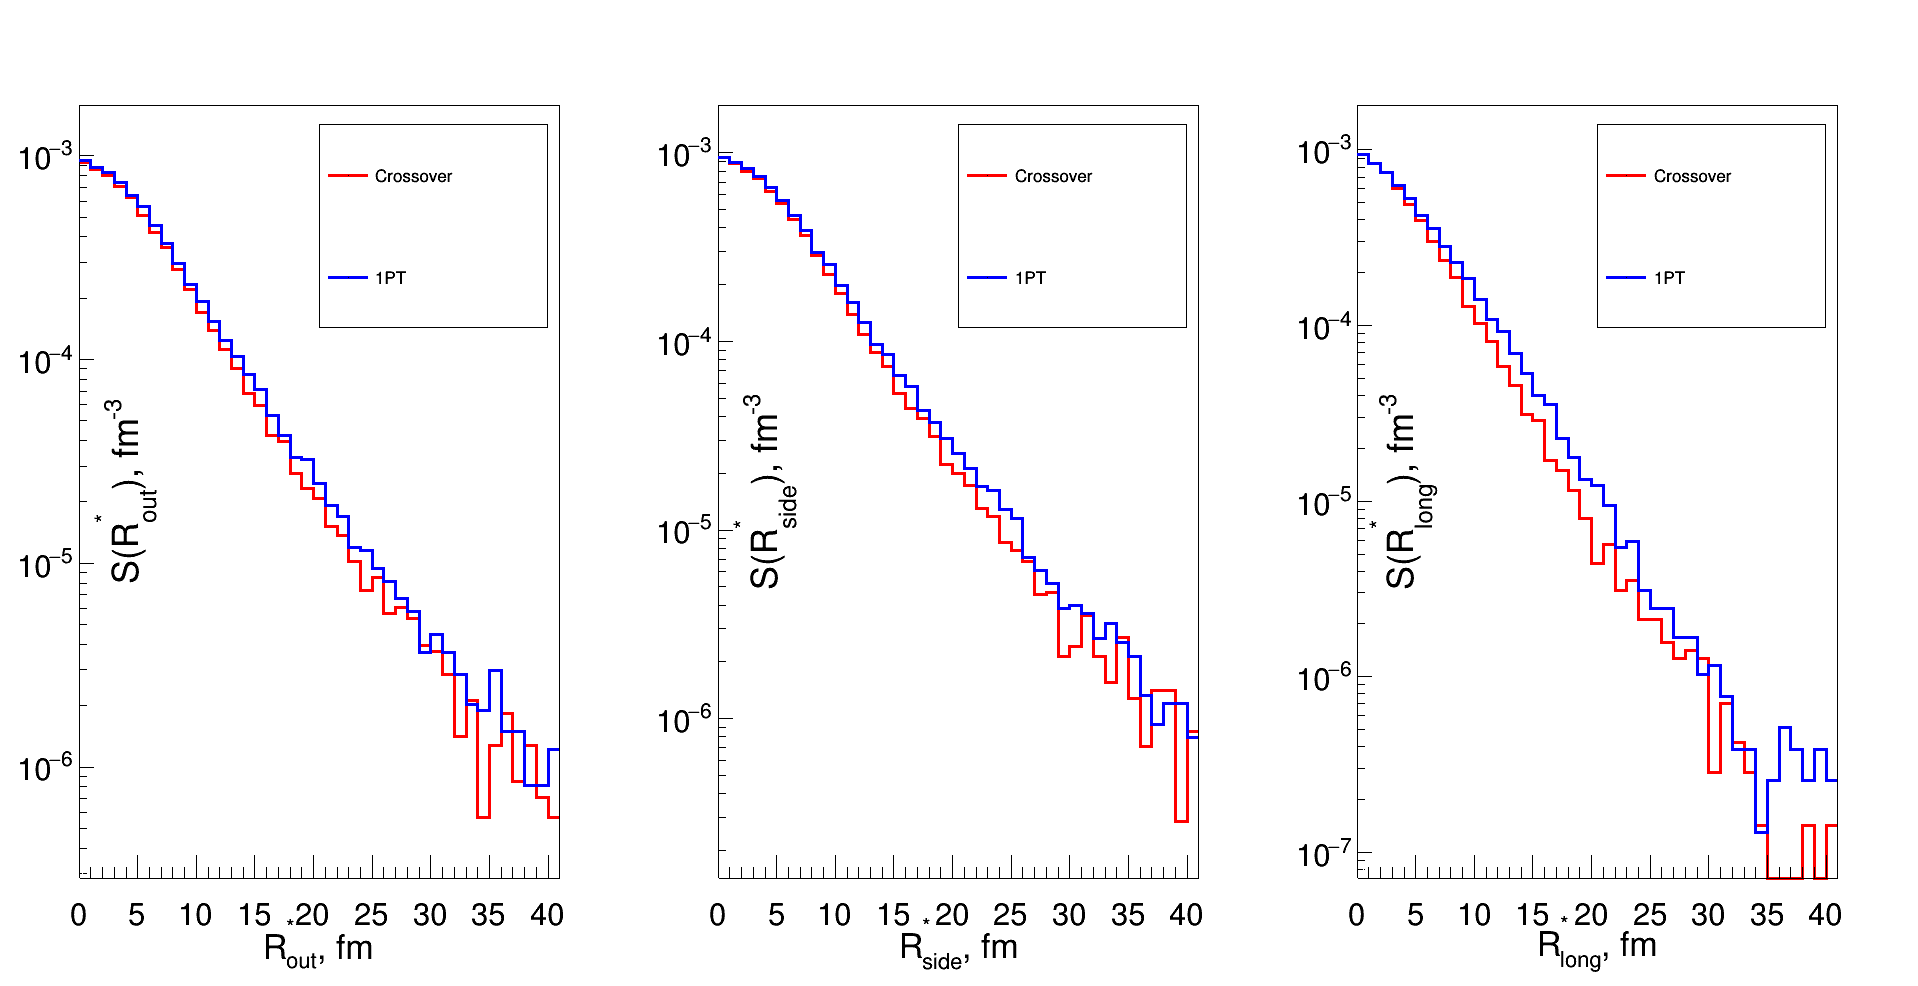
\includegraphics[width=1.\linewidth]{SF_vHLLE_UrQMD_115gev.png}
      \end{figure}
    \end{block}
  \end{columns}
  \note{
    In slide projections of the source function in the PRF on 
    out, side and longitudinal directions are presented.
    One may see that for calculations with the first order phase
    transition the visible tails of the source function are 
    longer than those obtained using crossover. The largest difference is seen in the long-direction,
    the effect becomes more visible with the increasing energy.
  }
\end{frame}

\begin{frame}
\frametitle{{\small \bf \centering Projections of Source Function, kaons (calculated in the PRF)}}	
\begin{block}{\bf \centering AuAu @ $\sqrt{s_{NN}} = 11.5$ GeV, vHLLE + UrQMD}
\begin{figure}[H]
        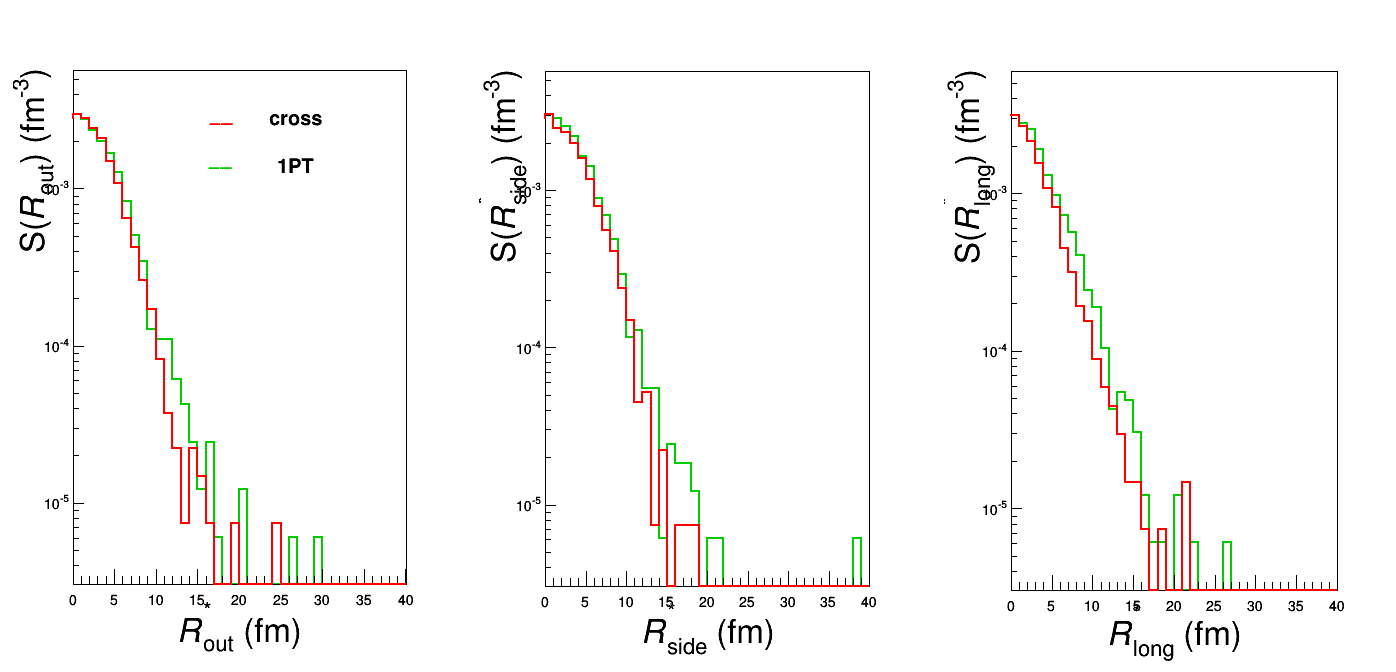
\includegraphics[width=1.\textwidth]{SF_115GeV_kaons.png}
      \end{figure}
	\end{block}
\end{frame}


\begin{frame}[shrink=35]
  \bf
  \frametitle{\bf \centering Simulation Framework for MPD (MPDROOT)} 
  \begin{columns}[c]
    \column{.60\textwidth}
    \begin{block}{}
      \begin{figure}[H]
        
\includegraphics[width=1.\textwidth]{mpdroot_web.png}
      \end{figure}
    \end{block}
    \column{.30\textwidth}
    \begin{block}{\bf \centering MPDROOT home web-page:}
      http://mpd.jinr.ru
    \end{block}
  \end{columns}
  \begin{columns}[c]
    \column{.20\textwidth}
    \begin{block}{}
      \begin{itemize}
      \item News
      \item Software repositories
      \item Software tests
      \item Forums
      \item Database for physics run
      \item E.t.c.
      \end{itemize}
    \end{block}
    \column{.33\textwidth}
    \begin{block}{}
      \begin{figure}[H]
        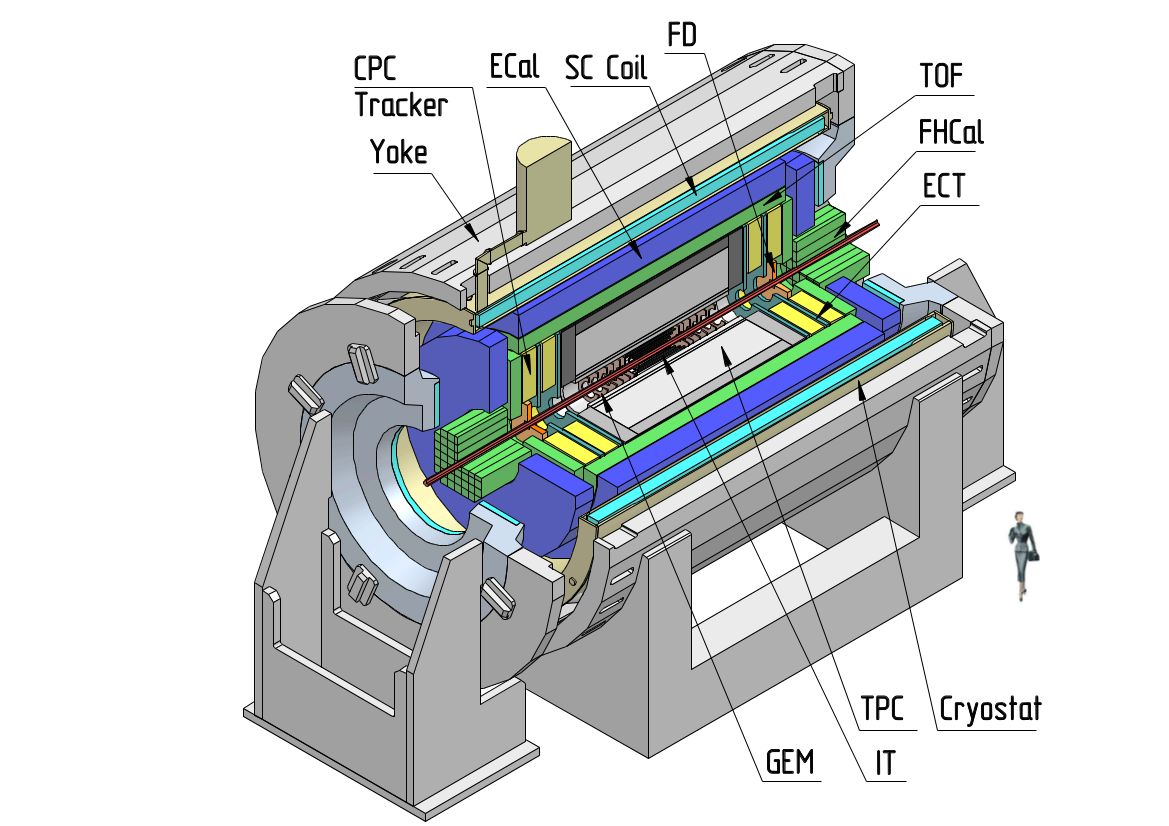
\includegraphics[width=1.\textwidth]{mpd.png}
      \end{figure}
    \end{block}
    \column{.40\textwidth}
    \begin{block}{\bf \centering Physics models to be used: }
      \begin{itemize}
      \item UrQMD / Hybrid UrQMD / vHLLE + UrQMD
      \item QGSM / LAGQSM
      \item HSD / PHSD
      \item 3FD
      \end{itemize}
    \end{block}
  \end{columns}
  \begin{columns}[c]
    \column{.10\textwidth}
    \column{.79\textwidth}
    \begin{block}{\bf \centering Benefits:}
      \begin{itemize}
      \item Inherits basic properties from FairRoot (developed at GSI), C++ classes
      \item Extended set of event generators for heavy-ion collisions
      \item Detector composition and geometry; particle propagation by GEANT3/4
      \item Advanced detector response functions, realistic tracking and PID included
      \item Event display for Monte-Carlo and experimental data 
      \end{itemize}
    \end{block}
    \column{.10\textwidth}
  \end{columns}
  \note{
  Since I am presenting a software group of the MPD experiment, I have to tell some words on the software we are using. Its main features are presented in the slide. It is built on C++ classes, allows one to perform simulations using an extended set of MC-generators presented in the slide. Also, it realizes propagation of particles through the detector and contains an event display to visualize Monte Carlo and experimental data. 
  }
\end{frame}

\begin{frame}[fragile, shrink=47]
  \bf 
   \frametitle{\bf \centering Femtoscopy within MPDROOT}
   \begin{columns}[c]
     \column{.4\textwidth}
     \begin{block}{\bf \centering NICAFEMTO}
       To be presented in the report of D.~Wielanek, GDRE 2016
     \end{block}
     \column{.4\textwidth}
     \begin{block}{\bf \centering {\color{red} FEMTOMPD} (is still developing)}
       Alternative software / package to perform femto-analysis within the MPDROOT
     \end{block}
   \end{columns}
   \begin{columns}[c]
     \column{.48\textwidth}
   \begin{block}{\bf \centering Example of macro to use within FEMTOMPD:}
     \begin{lstlisting}[language=C++,basicstyle=\ttfamily,keywordstyle=\color{red}]
       void femtoAna(...) {
           [ ... ] 
           MpdFemto* femto = new MpdFemto(...);
           femto->SetStartEvent(nStartEvent);
           femto->SetEvNumToRead(nEvents);
           femto->SetSourceSize(3.); 
           femto->SetPdgCode(211);
           femto->SetEtaCuts(-1.0, 1.0); 
           femto->SetPtCuts(0.15, 1.5); 
           femto->SetNumMixedEvents(10); 
           femto->SetKtCuts(0.15, 1.5); 
           femto->SetQinv(Qinv);
           femto->SetMagField(0.5); 
           femto->SetRadTpc(1.0);
           femto->SetMinNoHits(20);
           femto->SetZeroSharing(kTRUE);   
           // femto->SetQualityPairCut(kTRUE);
           femto->SetQualityMax(-0.4);
           femto->SetSharingMax(0.01);

           // A method to perform 1D-analysis
	       femto->MakeCFs_1D();
           [ ... ]
         }
     \end{lstlisting}
   \end{block}
   \column{.48\textwidth}
   \begin{block}{\bf \centering Benefits of the package: }
     \begin{itemize}
     \item totally integrated in the MPDROOT-software and based on the main principles of the MPDROOT (prev. slide)
     \item flexible due to consists of different modules to be expanded in a simple manner if necessary
     \item allows one {\color{red} to estimate influence of the two-track effects} (TTE) (splitting \& merging) in order to avoid distortion of CFs.
     \item 
     \end{itemize}
   \end{block}
   \begin{block}{\bf \centering HowTo:}
     http://mpd.jinr.ru/howto-install-mpdroot
   \end{block}
   \begin{block}{\bf \centering The MPD femto group:}
     \begin{itemize}
     \item Oleg Rogachevsky, \url{rogachevsky@jinr.ru}
     \item Ludmila Malinina, \url{Ludmila.Malinine@cern.ch}
     \item Konstantin Mikhaylov, \url{Konstantin.Mikhaylov@cern.ch}
     \item Daniel Wielanek, \url{daniel.wielanek@gmail.com}
     \item Pavel Batyuk, \url{pavel.batyuk@jinr.ru} 
     \end{itemize}
   \end{block}
   \end{columns}
   \note{
   At the moment, we have two packages in our software to perform femtoscopy analysis: NICAFEMTO to be presented in the report of D.~Wielanek and FEMTOMPD. It is an alternative package to perform analysis and its main features are presented in the slide. I would like to consider its application to an estimation of two-track effects, presented the next slide.
   }
\end{frame}

\begin{frame}
  \frametitle{Two Track Effects (TTE)}
  %\bf \centering N.B. It is put here as a temporary slide  
  \begin{columns}
    \column{0.48\textwidth}
    \begin{block}{\bf \centering Track merging}
      { \bf
        Two tracks that are spatially very close are falsely reconstructed as one.
        This will show up as an inefficiency of close pairs compared to a sample of unaffected pairs.
      }
    \end{block}
    \column{0.48\textwidth}
    \begin{block}{\bf \centering Track splitting}
      { \bf
        One track is falsely reconstructed as two tracks (or more).
        This will show up as an enhancement of close pairs compared to an uncorrelated sample.
      }
    \end{block}
  \end{columns}
  \begin{columns}
    \column{0.15\textwidth}
    \column{0.69\textwidth}
    \begin{block}{}
      {\bf 
        {\color{blue} CF could be affected by these effects} $\rightarrow$ \\
        {\color{red} shape of CF could be distorted}
      }
    \end{block}
    \column{0.15\textwidth}
  \end{columns}
  \note{
    The effects of hit sharing, track merging, track splitting are especially dangerous for analysis of femtoscopy correlations of identical particles at small relative momenta since CF could be affected these effects and its shape could be distorted. Explanation of the effects is presented in the slide and, probably, well known for majority of you.     
  }
\end{frame}

\begin{frame}
   \frametitle{\bf \centering TTE, details of analysis}
  \begin{block}{}
    \bf 
    The statistics used: $\sim$ 25 000 fully reconstructed events
    \\
    AuAu @ $\sqrt{s_{NN}}$ = 11.5 GeV,
    \\
    $\pi^{+}\pi^{+}$ pairs,

    % Centrality bins (\%): 0 - 50 

    $k_{T}$ bins ($ GeV/c $): 0.2 - 1.5
    
  \end{block}

  % \begin{block}{\bf Event Selection}
  %   \bf Reconstructed vertex $|V_{z}|$ < 8 cm
  % \end{block}

    \begin{block}{\bf \centering Single Track Cuts}
      \bf TPC tracks only
      
     \bf  $|\eta|$ < 1

      $ 0.2 < p_{T} < 1.5$ GeV/c

     $N_{hits}$ > 10 (maximal number of hits in a padrow per track is equal to 53)
    \end{block}

     \begin{block}{\bf \centering PID}
       \bf The PID MC was used for the analysis.
     \end{block}
     \note{In the slide I put details of the analysis.}
\end{frame}


\begin{frame}
  \bf
  \frametitle{\bf \centering Two Track Cuts}
  \begin{columns}[c]
     \column{.45\textwidth}
     \begin{block}{\bf \centering "Original'' CF}
       \begin{figure}[H]
        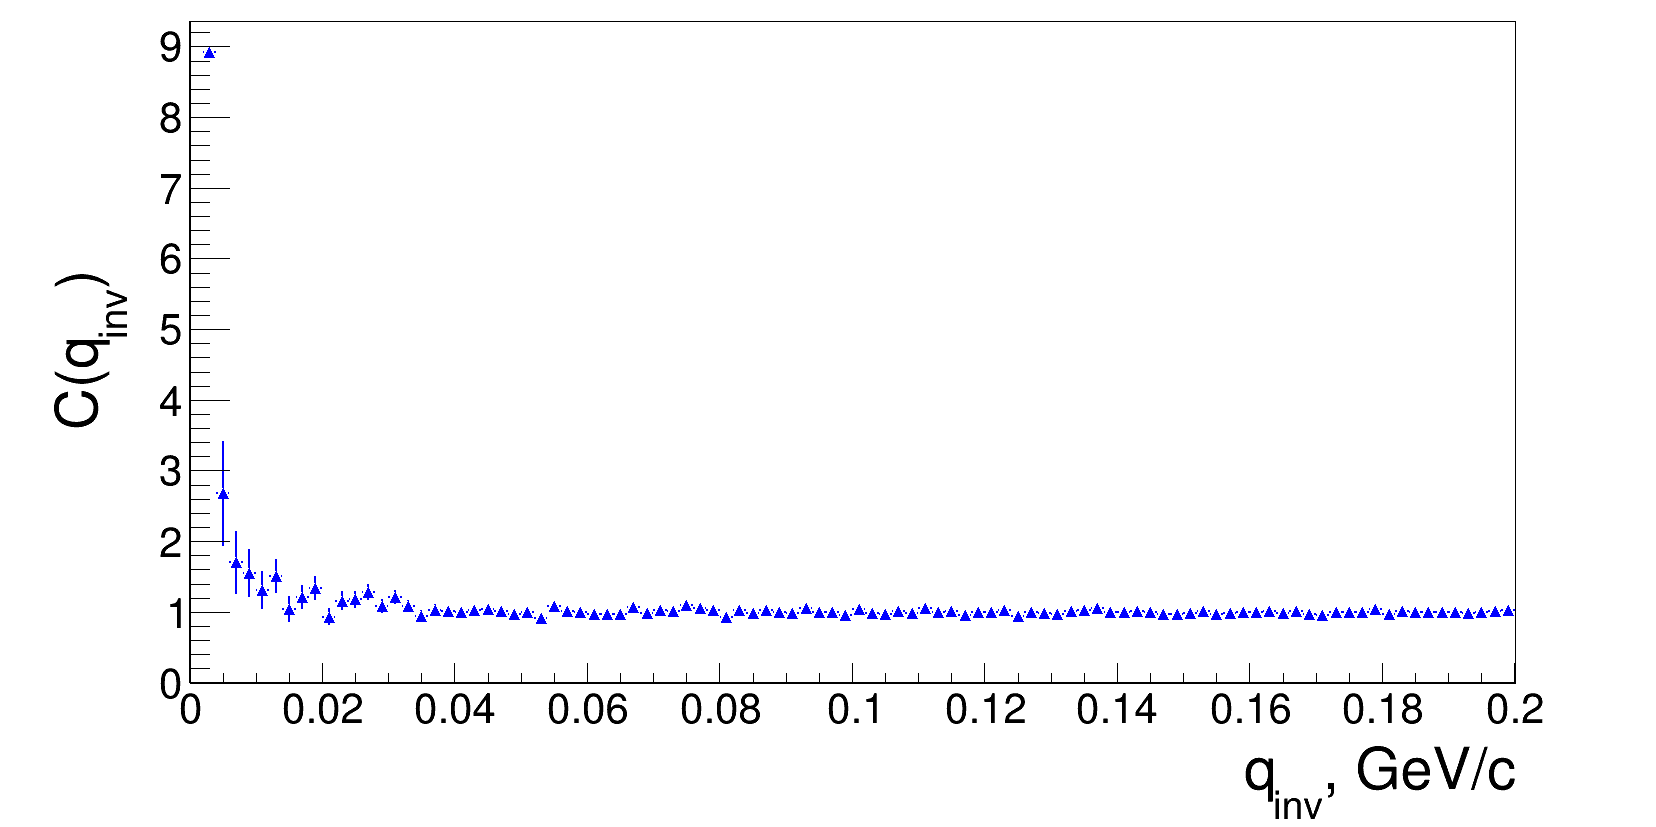
\includegraphics[width=1.\textwidth]{origCF_wo_suppression.png}
       \end{figure}
     \end{block}

     \column{.45\textwidth}
     \begin{block}{\bf \centering CF after splitting cut}
       \begin{figure}[H]
         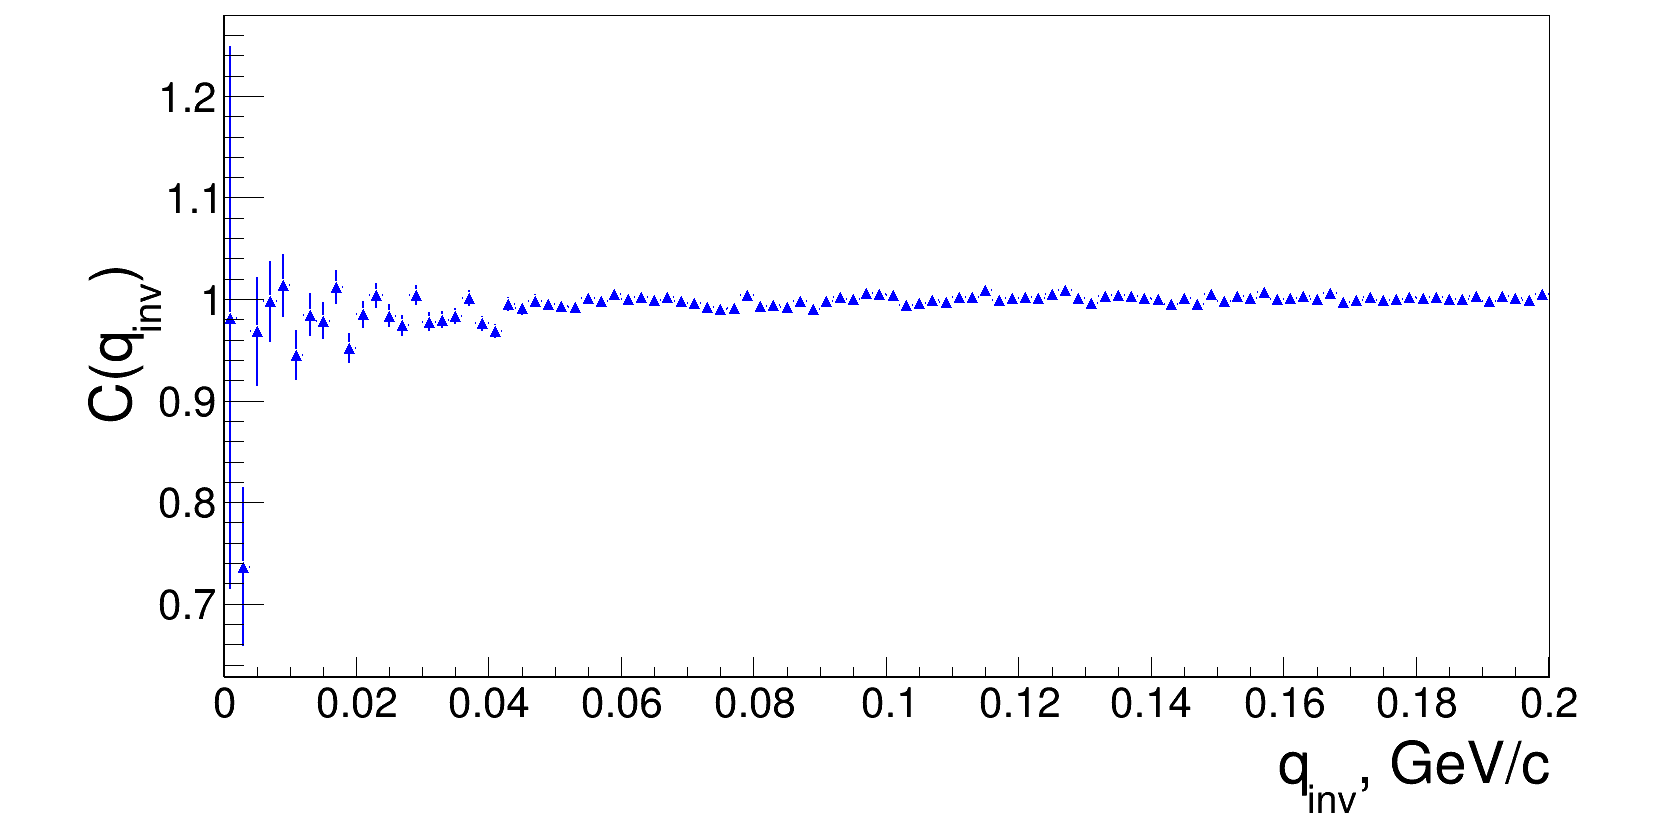
\includegraphics[width=1.\textwidth]{CFsAfterSplitSuppressed.png}
       \end{figure}
     \end{block}
  \end{columns}
  \begin{columns}[c]
    \column{.45\textwidth}
    \begin{block}{\bf \centering Fraction of splitting tracks}
       \begin{figure}[H]
        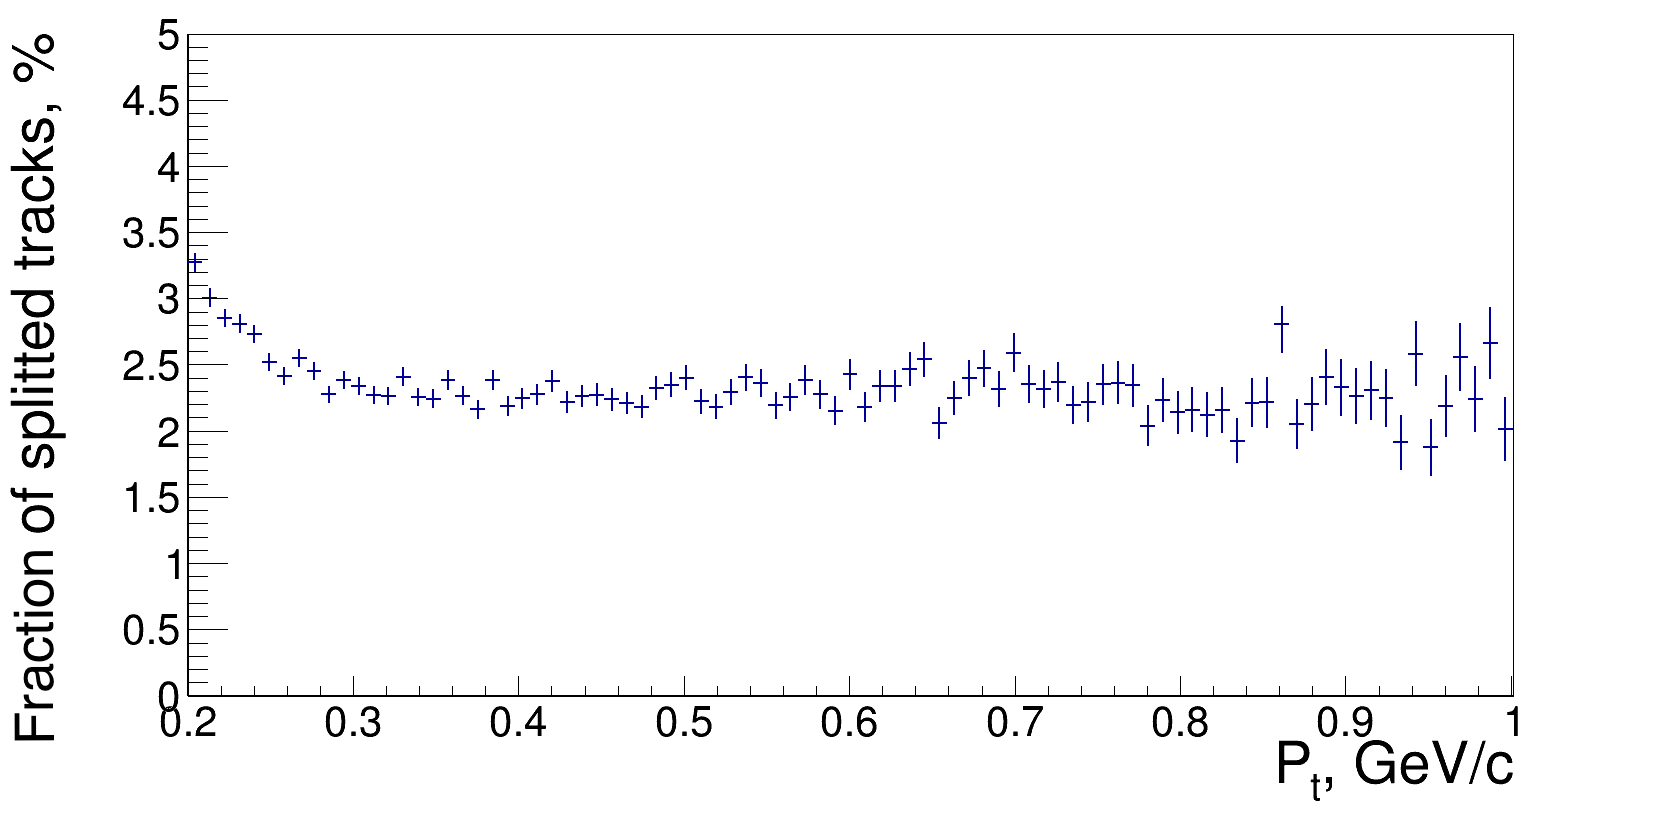
\includegraphics[width=1.\textwidth]{splitPionTracks.png}
       \end{figure}
     \end{block}
    \column{.45\textwidth}
    \begin{block}{\bf \centering Splitting: }
      \begin{itemize}
{\small
        \item reveals itself as a wide distribution with an average value of $\approx$ 2\% for $P_{t}$ = 0.3 - 1 GeV/c 
        \item affects sufficiently CFs
        \item is excluded nicely by use of (anti-)splitting cut
}
      \end{itemize}
    \end{block}
  \end{columns}
  \note{
  In the bottom row a distribution of fraction of splitting tracks depending on transverse momentum, is presented. One can see that the splitting reveals itself as a wide distribution with an averaged value of about 2\% starting from $P_{t}$ = 0.3 GeV/c. In the upper row two CFs are presented. Comparing them, one can see that the splitting distorts sufficiently form of the CFs.
  }
\end{frame}

\begin{frame}[shrink=50]
  \bf 
  \frametitle{\bf \centering Two Track Cuts}
  \begin{columns}[c]
    \column{.45\textwidth}
    \begin{block}{\bf \centering Quality cut}
      \begin{figure}[H]
        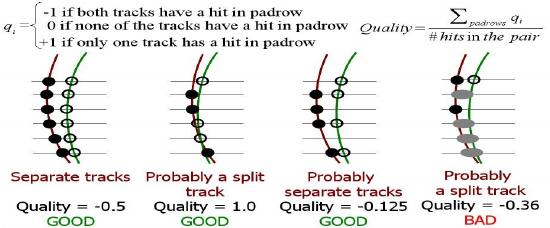
\includegraphics[width=1.\textwidth]{quality.png}
      \end{figure}
    \end{block}
    \begin{block}{\bf \centering Anti-merging cut}
      \begin{figure}[H]
        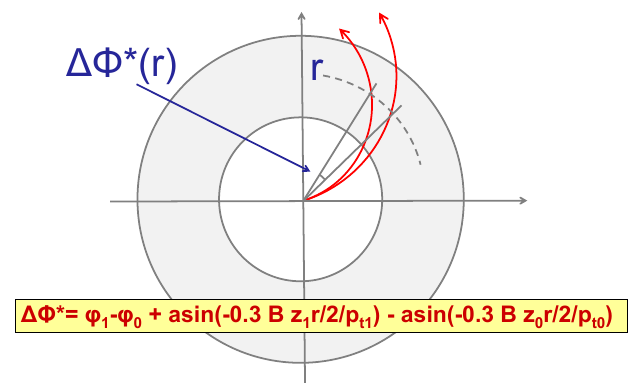
\includegraphics[width=1.\textwidth]{PhiStar.png}
      \end{figure}
    \end{block}
    
    \column{.45\textwidth}
    \begin{block}{\bf \centering Quality}
       \begin{figure}[H]
        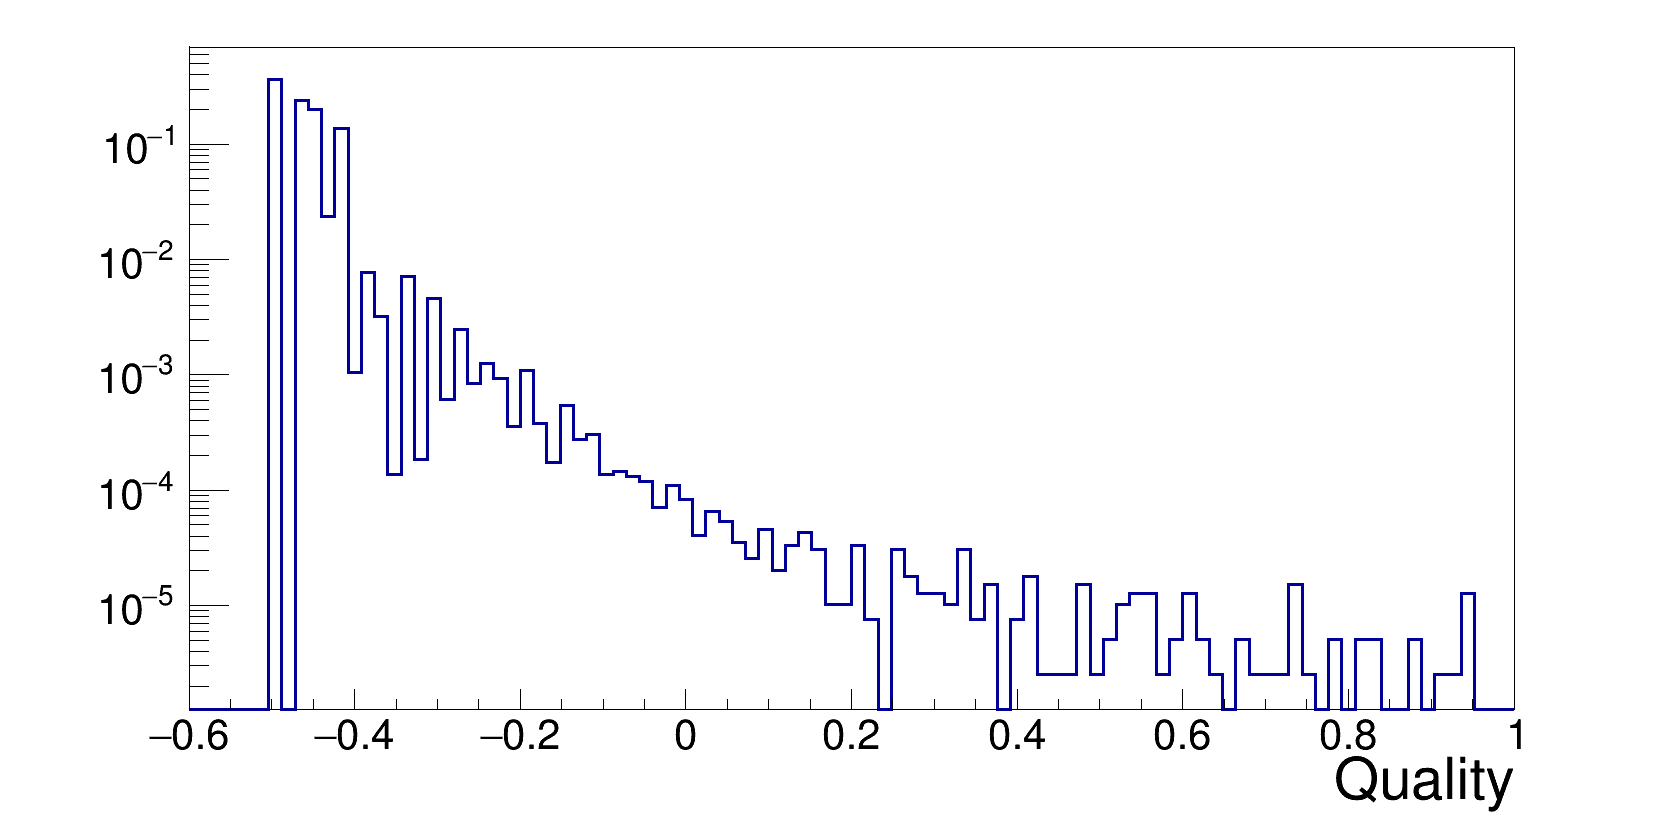
\includegraphics[width=1.\textwidth]{quality_distr.png}
      \end{figure}
    \end{block}
    \begin{block}{\bf \centering Sharing}
       \begin{figure}[H]
        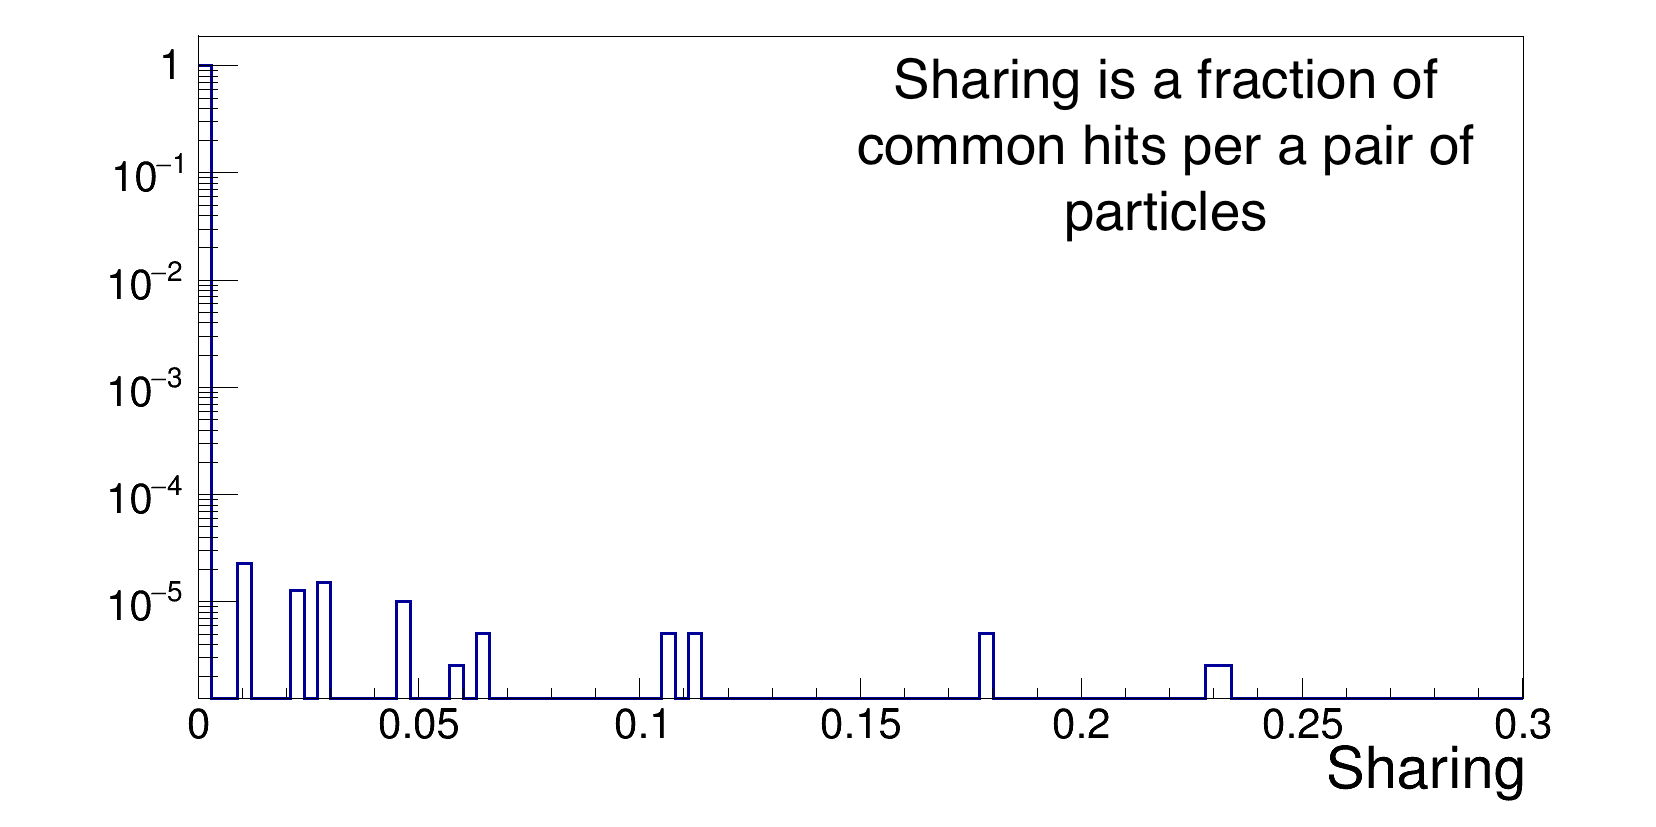
\includegraphics[width=1.\textwidth]{sharing_distr.png}
      \end{figure}
    \end{block}
%    \begin{block}{\bf \centering Quality vs. Sharing}
%      to be put here
%    \end{block}
  \end{columns}
  \begin{block}{}
    \begin{equation*}
      \Delta \Phi^{*}(R) = \phi_{1} - \phi_{0} + \arcsin \left(-\dfrac{0.3 B_{z} Z_{1} R}{2 P_{T1}}\right) - \arcsin \left(-\dfrac{0.3 B_{z} Z_{0} R}{2 P_{T0}}\right)
    \end{equation*}
        {\footnotesize
          $\phi_{1}$ and $\phi_{0}$ are azimuthal angles of the tracks at the vertex.
          
          $P_{T1}$ and $P_{T0}$ are their transverse momenta.
          
          $B_{z}$ indicates the magnetic field in z-direction.
          
          $Z_{1}$ and $Z_{0}$ are charges of particles forming the track.
        }
  \end{block}
  \note{After the splitting is considered to be excluded, the next step consists in estimation of the track merging. Its estimation can be done by analyzing quality and sharing distributions. Definitions of them are presented in the slide. It is possible to see that in our case the sharing does not look so crucial. One can observe a presence of the track merging using a special monitor distribution, called $\delta \eta \delta \phi^{*}$ and developed by the ALICE collaboration. A general definition of the cut is presented in the slide also.}
\end{frame}

\begin{frame}
  \bf 
  \frametitle{\bf \centering $d\eta d\Phi^{*}$ as a monitoring of TTE}
  \begin{columns}[c]
    \column{.45\textwidth}
    \begin{block}{\bf \centering $d\eta d\Phi^{*}$ (splitting cut used, no restriction on q, s = 0)}
     \begin{figure}[H]
        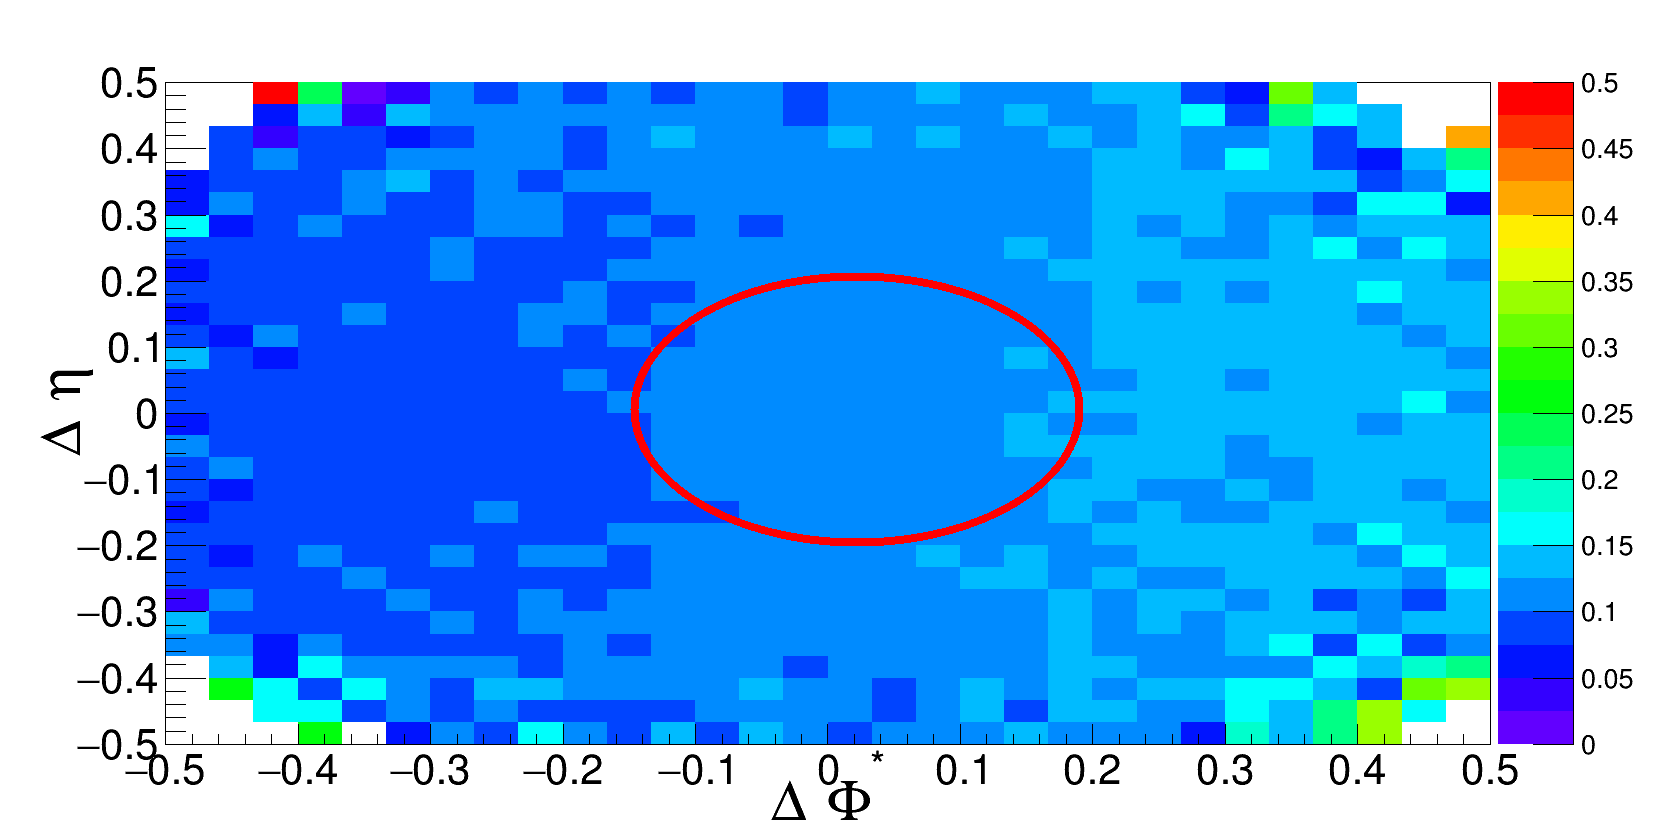
\includegraphics[width=1.\textwidth]{deltaPhiStarDeltaEta.png}
      \end{figure}
   \end{block}
    \begin{block}{}
      \bf \centering Probably, no merging?
    \end{block}
    \column{.45\textwidth}
    \begin{block}{\bf \centering $d\eta d\Phi^{*}$}
      \begin{figure}[H]
        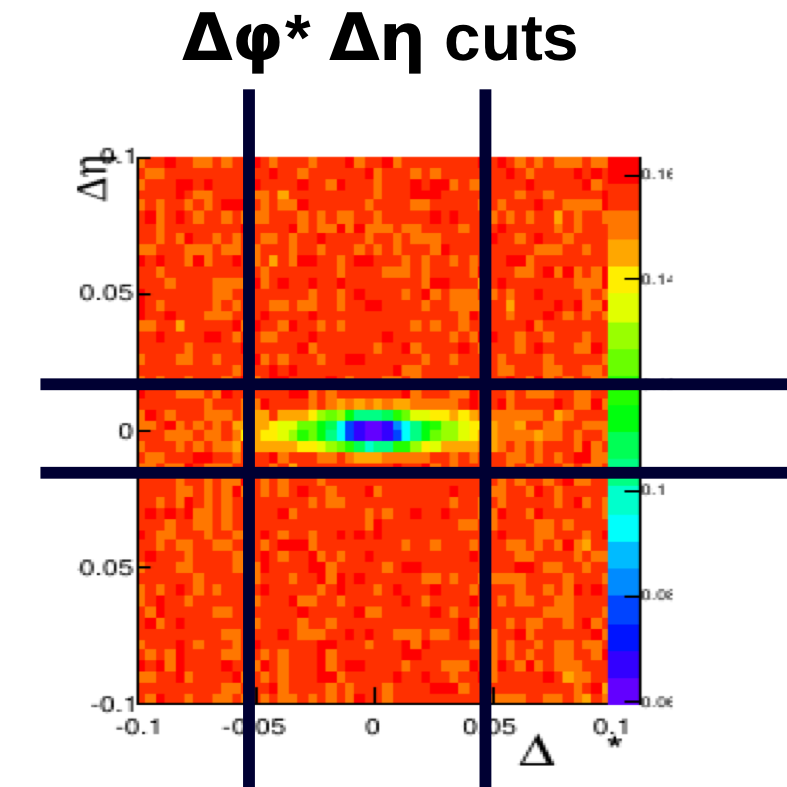
\includegraphics[width=1.\textwidth]{deltaEtadeltaPhi_howto.png}
      \end{figure}
   \end{block}
  \end{columns}
  \note{As possible to conclude from a comparison of the presented pictures $d\eta d\Phi^{*}$ did not reveal any track merging since we have no dip in the central region of the $d\eta d\Phi^{*}$-distribution.  This fact can be explained by different reasons. Among them, lack of statistics and an idealized algorithm of tracking procedure are considered as the candidates applied for explanation. Nevertheless, the question is still not closed and requires some additional efforts to be clarified.}
\end{frame}

\begin{frame}
  \bf 
  \frametitle{Conclusion \& Outline}
  \bf \centering 
  \begin{itemize}
  \item 1PT delays particle emission.  
  \item Obtained 3D CFs for pions and kaons appear to be sensitive to different EoS's.
  \item We plan to study the non-Gaussian tails of CFs using the Hump parametrization.
  \item Despite hadronic cascade affects strongly the observed source functions, it looks possible to distinguish them within the vHLLE + UrQMD hybrid model.
  \item We plan to continue studies with larger statistics for $\pi$- and $K$-mesons.
  \item A study of TTE within the FEMTOMPD has been done
 and is planned to be continued.
  \end{itemize}
 \note{
 Here, I am going to the conclusions.
 }
\end{frame}



%% BACKUP SLIDES
\begin{frame}
  \bf
  \frametitle{\bf \centering BACKUP SLIDES}
\end{frame}

\begin{frame}[shrink=33]
  \bf
  \frametitle{{\small \bf \centering vHLLE + UrQMD, $\sqrt{s_{NN}} = 11.5$ GeV, projections of the 3D CF, pions}}
  \begin{block}{\centering \bf EoS: 1-st order phase transition (1PT)}
    \begin{figure}[H]
       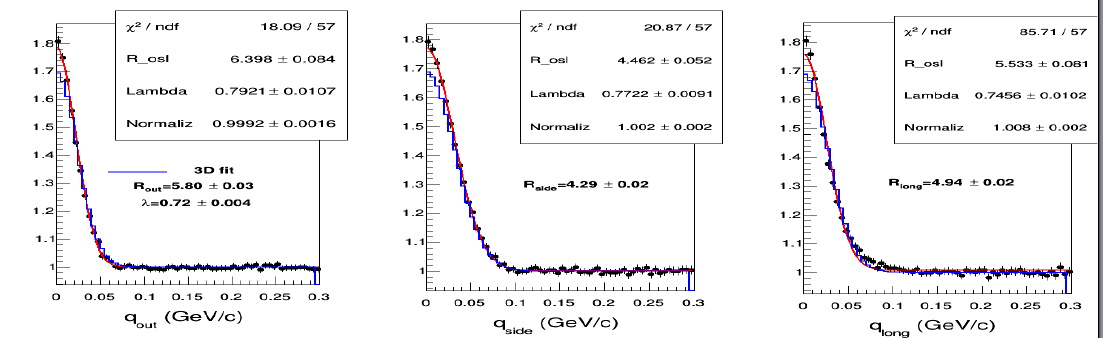
\includegraphics[width=1.\textwidth]{3DCF_projections_1pt.png}
     \end{figure}
  \end{block}
  \begin{columns}[c]
    \column{.48\textwidth}
    \begin{block}{}
      \begin{itemize}
      \item Gaussian fit of the CFs does not describe shape of the CFs at small $\bf q$.
      \item A difference observed between the 3D CFs fit and a fit of 1D projections of the 3D CFs leads to a conclusion
        that the projections look more Gaussian. 
      \item $R_{out}$ and $R_{long}$, obtained in case of 1PT, are larger than the ones in case of the crossover EoS.
      \end{itemize}
    \end{block}
    \column{.48\textwidth}
    \begin{block}{}
      \begin{itemize}
      \item Difference between the 1PT and crossover EoS's is small. The maximum difference is observed for $R_{long}$.
      \item {\color{red} Non-Gaussian fits will be tried.}
      \item {\color{red} CFs for kaons will  be studied.}
      \end{itemize}
    \end{block}
  \end{columns}
\end{frame}




  

\end{document} 
